\documentclass[manual,palatino,fontecodigo,codigo,glenn,refnum]{Estilo}
%%%
%%% \KOMAoption{headsepline}{0pt} %descomente para retirar a linha do cabeçalho
%%%
%%%-----------------------------------------------------------------------------
%%%
%%% Início do documento
%%%
\begin{document}
%%%
\frontmatter %%% Necessário para os ajustes da parte pre-textual
%%%
%%% Capa
%%%
\thispagestyle{empty}
\imagemsl{Logorural}

\vspace*{6cm}
\begin{center}
   {
   \scshape\huge Classe Estilo\vspace*{-0.35cm}
   \noindent\rule{\textwidth}{3pt}
   }
   {
   \Large\artemisia Trabalhos acadêmicos em \LaTeX\ de acordo com as
   normas de formatação do curso de Matemática\vspace*{-0.35cm}
   }
   \noindent\rule{\textwidth}{3pt}
\end{center}
\vspace{6.5cm}

\begin{center}
	Benaia Sobreira de Jesus Lima\\
	\today\\
    \textcolor{estilo}{{\scshape Versão 1}}
\end{center}
%%%
%%% Fim da capa
%%%
\tableofcontents    %%% Sumário
%%%\listoffigures   %%% Lista de figuras
%%%\listoftables    %%% Lista de tabelas
%%%
\introducao

Ainda que possível, digitalizar e depois imprimir um documento não é o método
adequado para obter uma cópia, para esse propósito existem instrumentos específicos e adequados, as máquinas de reprografia. Para cada tarefa há uma ferramenta adequada.

Em matemática a redação de texto em geral exige a inclusão de gráficos, imagens, símbolos, caracteres gregos, equações, fórmulas, enumeração desses elementos e referências cruzada a eles. O sistema \TeX$\backslash$\LaTeX\ é uma ferramenta
apropriada para manipular e/ou construir esses elementos.

A classe estilo usa o sistema \TeX$\backslash$\LaTeX\ e foi concebida para ser um
instrumento adequado para a construção de trabalhos acadêmicos/científicos de acordo com as normas de formatação do curso de Matemática do Departamento de Tecnologias e Linguagens - DTL.

\section*{O que é a classe Estilo?}

A classe \estilo\ é uma extensão da classe \ttt{scrbook}, que é parte do koma-script. Sua adoção não é obrigatória, apenas é muito incentivada.

\section*{Por que usar a classe Estilo?}

Para não se preocupar com normas de formatação, concentrar-se no conteúdo e
aproveitar todos os benefícios que o \LaTeX\ oferece para a edição
de teorema, fórmulas, equações, imagens, e outros. Para construir documentos tipograficamente coerentes, organizados e inserir elementos tipográficos como capa, folha de rosto, sumário, notas de rodapé, anexos, apêndices e outros
de forma intuitiva e simples, com um único comando ou ambiente.

\ajuste %%% necessário 

\chapter{Classe Estilo: aquisição e uso}


\section{Aquisição}

Para obter a classe \estilo\ envie e-mail para

\begin{center}
	\ttt{\textcolor{estilo}{matematica.ufrrjim@gmail.com}}
\end{center}
e a solicite. Você receberá um e-mail resposta com o arquivo
Estilo.rar\footnote{Esse é um arquivo compactado pelo Winrar,
deve ser aberto pelo Winrar, winzip ou equivalentes, como
o brazip por exemplo.} anexo, descompacte-o em  qualquer
pasta.

Ao descompactar o \ttt{Estilo.rar} você encontrará o manual (pdf) da 
classe estilo e a pasta Monografia, essa pasta contém:
\begin{description}
    \item[Imagens:] pasta contendo imagens utilizadas como exemplo;
    \item[Estilo.cls:] arquivo com todas as definições da classe \estilo;
    \item[logotipo.tex:] utilizado para inserir a logomarca da instituição;
    \item[Logo.png:] logomarca da UFRRJ em \ttt{.png};
    \item[Bibliografia:] Exemplo de banco bibliográfico segundo as regras
	    do Bib\TeX.
    \item[MonoExemplo:] um exemplo de monografia.
\end{description}


% % % \section{Instalação}
% % % 
% % % A classe \estilo\ não exige instalação para ser utilizada,
% % % basta colocar seu arquivo \ttt{.tex} na mesma pasta do
% % % arquivo \estiloc. 
% % %
% % % Contudo, uma instalação permite que a
% % % classe seja utilizada sem que seu arquivo .tex esteja na mesma
% % % pasta do arquivo \estiloc.
% % % 
% % % A instalação consiste em fazer a classe visível ao sistema
% % % TeX/\LaTeX, para isso abra uma pasta(com qualquer nome) no
% % % diretório de instalação do seu sistema \TeX/\LaTeX, ponha o
% % % arquivo \estiloc\ dentro dessa pasta e atualize o FNDB de
% % % sua distribuição, simples assim. Se não sabe o que é FNDB
% % % não tente instalar a classe estilo, use-a sem instalação e
% % % esteja seguro de que não vai correr o risco de bagunçar o
% % % seu sistema.

\section{Utilização}

A classe \estilo\ não exige instalação para ser utilizada,
basta colocar seu arquivo \ttt{.tex} na mesma pasta do
arquivo \estiloc. 

A estilo foi concebida para atender satisfatoriamente o usuário com pouca ou 
nenhuma experiência em \LaTeX. Para utilizá-la defina a primeira linha de 
seu arquivo \ttt{.tex} da seguinte forma

\begin{center}
   \cmc{documentclass}{Estilo}
\end{center}

Assim como as classes tradicionais, a \estilo\ admite parâmetros opcionais 
com os quais é possível alterar e/ou adicionar características e 
funcionalidades. Esses parâmetros são as opções de classe e estão 
descritas na seção \ref{opce}. Sua sintaxe é:

\begin{center}
	\cmco{documentclass}{opção 1, opção 2,$\ldots$}{Estilo}
\end{center}

Para compilar use os mesmos métodos utilizados com as classes nativas do \LaTeX.


\chapter{Características da classe Estilo}


\section{Espaço entre linhas}\label{entrelinha}

Na classe \estilo\, o controle do espaço entre linhas é feito pelo pacote \paco{setspace} e o espaçamento padrão é um e meio, dado pela opção \ttt{onehalfspacing}.

\section{Margens e tipo de papel}\label{margens}

O controle das margens é feito com o pacote \paco{geometry}. O papel padrão na classe \estilo\ é o A$4$, definido por meio da chave a4paper. As margens e o tipo de papal são definidas pelo comando
\begin{center}
	\cmc{geometry}{a4paper,\epar{inner}{4cm},\epar{outer}{3cm},
	     \epar{top}{3cm},\epar{bottom}{2cm}}
\end{center}
Isto quer dizer que
\begin{multicols}{2}
\begin{itemize}
	\item Margem esquerda $=4$ cm
	\item Margem direita $=3$ cm
	\item Margem superior $=3$ cm
	\item Margem inferior $=2$ cm
\end{itemize}
\end{multicols}

\section{Pacotes sempre carregados}

Algumas pacotes sempre são carregados pela classe \estilo, outros ficam 
acessíveis apenas quando uma opção de classe é fornecida. Os pacotes 
sempre carregados são os seguintes:
\begin{description}
   \item[\upacoo{utf8}{inputenc}:] codificação unicode, permite inserir os 
   caracteres acentuados e ç diretamente pelo teclado.
   \item[\upaco{geometry}:] ver~\ref{margens}.
   \item[\upacoo{TS1,T1}{fontenc}:] condificação da fonte de saída, a codificação padrão é T1.
   \item[\upacoo{brazil}{babel}:] traduz para português muitos termos
        produzidos pelo \LaTeX.
   \item[\upaco{scrhack}:] o KOMA usa seu próprio algoritmo para criar
        ambientes flutuantes fornecidos pelo tocbasic. Portanto, pacotes
        como float ou listings usam uma versão antiga e produzem avisos.
        No entanto, Markus Kohm escreveu um pequeno pacote chamado scrhack
        que corrige esse problema. Como os pacotes float e listings são carregados
        pelas opções imagem (padrão) e codigo, foi necessário carregar esse pacote
        na \estilo.
   \item[\upacoo{onehalfspacing}{setspace}:] ver~\ref{entrelinha}.
   \item[\upaco{fix-cm,etex,xspace e calc}:] pacotes técnicos e utilitários carregados sem
   	    qualquer opção.
   \item[\upaco{xcolor}:] suporte a cor. É carregado com as opções
        svgnames, table, x11names, dvipsnames e hyperref.
   \item[\upaco{microtype}:] melhorias para as fontes. É carregado com as opções
        final,kerning,babel,protrusion=true,expansion=true e tracking=true
   \item[\upaco{hyperref}:] utilitário, ver~\ref{links}.
   \item[\upaco{bookmark}:] utilitário
   \item[\upacoo{figure}{hypcap}:]  utilitário
   \item[\upaco{caption}:] formata a legenda de figuras e tabelas criadas
        dentro dos ambientes figure e table. É carregado com as opções
        labelfont=$\{$small,bf,s$\}$, font=$\{$small,sf$\}$, hypcap=false.
   \item[]\cmc{captionsetup}{\epar{justification}{centering}}: legendas de figuras e
        tabelas centralizadas
   \item[\upaco{subcaption}:] ajuda na formatação das legendas.
   \item[\upaco{textcomp}:] fonte, ajustes e símbolos com o encode TS1.
   \item[\upaco{cancel}:] simplificação (cancelamento) de expressões.
   \item[\upaco{rotating}:] suporte para girar coisas.
   \item[\upaco{boxedminipage}:] minipáginas com moldura
   \item[\upaco{makeidx}:] para criar índice remissivo
   \item[\upaco{wallpaper}:] imagem em plano de fundo
   \item[\upaco{multicol}:] conteúdo em mais de uma coluna
   \item[\upaco{amsmath,wasysym,amsfonts,amssymb,amstext}]
   \item[\upaco{amsthm,fixmath}:] demandas variadas em matemática
   \item[\upaco{thmtools}:] utilizado para definir os ambientes para teorema,
               definição, exemplo, corolário, e outros.
   \item[\upaco{enumitem}:] utilitário para listas, foi utilizado para definir
               ajustes para os ambientes enumerate, itemize e description.
   \item[\upaco{float,graphicx}:] carregados por meio da opção \op{imagem} que é padrão.
               O float define o posicionar H e o graphicx permite inserir imagens....  
\end{description}


\section{Estrutura do Documento}

O \LaTeX\ e a classe \estilo\ permite dividir o documento em
parte, capítulo, seção, subseção, subsubseção e parágrafo.
\begin{tcolorbox}
\begin{tabular}{lcl}
   Parte       &$\longrightarrow$& \cmc{part}{título da parte} \\
   Capítulo    &$\longrightarrow$& \cmc{chapter}{título do capítulo} \\
   Seção       &$\longrightarrow$& \cmc{section}{título da seção} \\
   Subseção    &$\longrightarrow$& \cmc{subsection}{título da subseção} \\
   Subsubseção &$\longrightarrow$& \cmc{subsubsection}{título da subsubseção}\\
   Parágrafo   &$\longrightarrow$& \cmc{paragraph}{título do parágrafo}
  \end{tabular}
\end{tcolorbox}

\begin{tcolorbox}[title={Classe estilo: estrutura de um documento científico}]
\begin{lstlisting}
\documentclass{Estilo}

\autor{nome do autor}
\title{título do trabalho}

\begin{document}
   \frontmatter
      Parte pré-textual
   \introducao % fim da parte pré-textual. Inclui \mainmatter

      Conteúdo da introdução

   \ajustes % fim da introdução

      Parte textual

   \bibliographystyle{um estilo de bibliografia}
   \bibliography{nome do arquivo}
\end{document}
\end{lstlisting}
\end{tcolorbox}

\section{Opções da classe Estilo}\label{opce}

A implementação preservou todas as \op{opções} da classe base \ttt{scrbook}.
As opções padrão atendem a todas as normas de formatação de trabalhos científicos do curso de Matemática do Departamento de Tecnologias
e Linguagens - DTL. Além das opções da classe \ttt{scrbook} a classe \estilo\
admite opções próprias, as quais seguem.

\begin{description}
\item[latin:] carrega \upacoo{latin1}{inputenc} e dessa forma ativa suporte à
   codificação iso.
\item[unicode \opp{(padrão)}:] carrega \upacoo{utf8}{inputenc} e dessa forma
   ativa suporte à codificação unicode.
\item[imagem \opp{(padrão)}:] essa opção carrega os pacotes \pacote{float} e
   \pacote{graphicx} e vem ativa por padrão. Podem ser incluídas imagens
   em todos os formatos que o \LaTeX\ aceita, tais como
   \ttt{.png, .pdf, .jpg, .mps (METAPOST)} e outros.
\item[licenciatura \opp{(padrão)}:] ajusta {\sffamily capa} e {\sffamily folha
   de rosto} para uma monografia de graduação relativa a um curso de  licenciatura;
\item[bacharel:] ajusta {\sffamily capa} e {\sffamily folha de rosto}
   para uma monografia de graduação relativa a um curso de bacharelado;
\item[especialista:] ajusta {\sffamily capa} e {\sffamily folha de rosto}
   para uma monografia de curso de especialização;
\item[mestre:] ajusta {\sffamily capa} e {\sffamily folha de rosto} para
   uma dissertação de mestrado;
\item[doutor:] ajusta {\sffamily capa} e {\sffamily folha de rosto} para
   uma tese de doutorado.

\item[Enumeração das páginas:] A enumeração padrão é a da classe
    \textrm{scrbook} e não depende de nenhum pacote. A classe \estilo\
    utiliza o pacote \paco{scrlayer-scrpage} para disponibilizar, na
    forma de opções de classe, cinco tipos de enumeração de páginas, são elas:
    \begin{center}
        \ttt{sofisticada, completa, popular, popularsec, secpopular}
    \end{center}
     Ao utilizar uma dessas opções deve-se
    \begin{enumerate}
    	\item criar a introdução com o comando \com{introducao}.
    	\item finalizar a introdução com o comando \com{ajuste}.
    \end{enumerate}
    Esses comandos ajustam as definições internas e asseguram enumeração correta da parte \emph{textual}.

      \begin{description}
      \item[sofisticada:] todas as páginas são contadas, mas enumeradas a partir na segunda página do sumário com enumeração no cabeçalho, que também recebe uma linha contínua. O rodapé é vazio e a primeira página dos capítulos não recebe numeração. Parte pré-textual enumerada em algarismos romanos as demais em arábicos.
      \begin{itemize}
      	\item se a opção \op{oneside} é carregada(impressão simples, anverso,
      	     apenas frente) o número da página será alinhado à esquerda com o número e título do capítulo alinhados à direita.
      	\item se a opção \op{twoside} é carregada(impressão frente e verso)
      	     o cabeçalho das páginas ímpares terá o número da página alinhado à esquerda com número e título da seção mais próxima alinhados à direita. O cabeçalho das páginas pares terá o número da página alinhado à direita com número e título do capítulo alinhados à esquerda.
      \end{itemize}
      \item[completa:] difere da opção \ttt{sofisticada} somente por enumerar, também, a página inicial dos capítulos e das estruturas definidas a partir do comando \comando{chapter}, como o sumário, lista de tabelas, figuras,$\ldots$;
      \item[popular:] todas as páginas são contadas, mas enumeradas a partir na segunda página do sumário com enumeração no cabeçalho, que também recebe uma linha contínua. O rodapé é vazio e a primeira página dos capítulos não recebe numeração. Parte pré-textual enumerada em algarismos romanos as demais em arábicos.
      \begin{itemize}
      	\item se a opção \op{oneside} é carregada(impressão simples, anverso,
      	apenas frente) o número da página será alinhado à direita com o número e título do capítulo alinhados à esquerda.
      	\item se a opção \op{twoside} é carregada(impressão frente e verso)
      	o cabeçalho das páginas ímpares terá o número da página alinhado à direita com número e título da seção mais próxima alinhados à esquerda. O cabeçalho das páginas pares terá o número da página alinhado à esquerda com número e título do capítulo alinhados à direita.
      \end{itemize}
      \item[popularsec\opp{(padrão)}:] difere da opção \ttt{popular} apenas em documento para impressão simples (opção oneside). A diferença consiste em substituir, no cabeçalho, o título do capítulo pelo título da seção atual;
      \item[secpopular:] difere da opção \ttt{sofisticada} apenas quando a opção \op{oneside} e carregada, ou seja, documento para impressão simples. Nesse caso o número da página é alinha à esquerda e o número e título da seção mais próxima alinhados à direita.
    \end{description}
\item[refkoma\opp{(padrão)}:] referência padrão da classe \ttt{scrbook}.
\item[refnum:] referência numérica.
\item[refaa:] referência autor-ano.
\item[codigo:] carrega o pacote \pacote{listings} e suas ferramentas para 
inserir código, veja os detalhes no capítulo~\ref{codigos}, essa opção é 
desnecessária se for utilizada a opção \op{timesH}. A fonte padrão do código é 
a mesma do texto mas com a família \com{ttfamily}, as opções \op{courier} e 
\op{fontecodigo} permiter alterar e fonte do código.
\item[courier:] carrega \upaco{courier} e deve ser usada preferencialmente em 
conjunto com a \op{timesH} pois altera outras fontes além da fonte dos códigos. 
\item[fontecodigo:] sem carregar \upaco{courier}, altera a fonte do código para 
courier.
\item[palatino:] disponibiliza as seguintes fontes
\begin{itemize}
	\item \upacoo{scaled=.88}{beramono} fonte Bera Monoespaçada.
	\item \upacoo{scaled=.86}{berasans} fonte Bera sem serifa.
	\item \upacoo{sc,osf}{mathpazo} fonte Palatino com small caps e números pequenos.
\end{itemize}
\item[artemisia:] \upaco{gfsartemisia-euler} fonte artemisia.
\item[lmoder:] \upaco{lmodern,libertine} fonte lmodern + libertine (linux)
\item[timesA:] fonte Adobe Times Roman para o corpo do texto e Avantegarde para 
os títulos. Carrega os pacotes \upaco{mathptmx} e \upaco{avant} e utiliza  os 
símbolos matemáticos das fontes Symbol, Chancery e Computer Modern.
\item[timesH:] fonte Times-Helvetica-Courier com os pacotes
\begin{itemize}
	\item \upaco{mathptmx}
	\item \upacoo{scaled=0.92}{helvet}
	\item \upaco{courier}
\end{itemize}
\item[lsec:] essa opção muda o posicionamento dos números das seções e 
subseções. Ative-a, compile e aprecie.
\item[apenas:] permite a criação de apêndices sem anexos.

\item[Página inicial dos capítulos:] a classe estilo disponibiliza cinco opções
    de formatação da página inicial dos capítulos, sumério, referências, anexos e apêndices.
    \begin{description}
    	\item[sonny:] carrega \upacoo{Sonny}{fncychap}
    	\item[lenny:] carrega \upacoo{Lenny}{fncychap}
    	\item[glenn:] carrega \upacoo{Glenn}{fncychap}. Essa opção é incompatível com \epar{bibliography}{totoc} que insere a entrada das referências no sumário, quando carregadas juntas não é criado o retângulo que envolve o título das referências. Assim, quando a opção glenn é carregada a classe estilo não carrega a opção \epar{bibliography}{totoc}, por isso é necessário inserir manualmente a entrada da referências no sumário, o que é feito pondo o comando
    	\begin{tcolorbox}
    	\begin{lstlisting}
    	   \addcontentsline{toc}{chapter}{Referências}
    	\end{lstlisting}
    	\end{tcolorbox}
    	acima do \com{bibliographystyle}. Essa é uma peculiaridade exclusiva da opção glenn.
    	\item[conny:] carrega \upacoo{Conny}{fncychap}
    	\item[rejne:] carrega \upacoo{Rejne}{fncychap}
    	\item[bjornstrup:] carrega \upacoo{Bjornstrup}{fncychap}
    \end{description}
\end{description}

\section{Indentação}

A classe \estilo\ indenta todos os parágrafos,
inclusive o primeiro, seja ele de capítulo, seção ou subseção.

\chapter{Identificação do trabalho}\label{identifica}

Várias informações para identificação do trabalho, composição da
banca examinadora, data, identificação da instituição, cidade e
outras são requeridas para compor a versão final. Na classe \estilo,
para cada uma dessas informações há um comando específico que deve
ficar no preâmbulo. Se um ou mais desses comandos não for declarado
um valor padrão é assumido ou é exibida uma mensagem avisando ao
autor sobre o esquecimento daquela informação.

\section{Instituição}

\subsection{Logomarca}

A classe \estilo\ constrói a capa independente da existência de
uma logomarca. Porém, adicionando os arquivos \ttt{logotipo.tex}
e \ttt{Logo} à mesma pasta de seu arquivo \ttt{.tex} a imagem
contida no arquivo \ttt{Logo} será inserida sobre o nome da instituição.

O arquivo \ttt{Logo} deve está em um dos formatos:
\ttt{.ps, .eps, .png, .pdf, .jpg}. O \ttt{logotipo.tex} é distribuído
com a classe \estilo\ e é o responsável pela inclusão e formatação da imagem.

Se for necessário alterar o tamanho da imagem abra o arquivo
\ttt{logotipo.tex}, o parâmetro \ttt{scale} controla o tamanho da
imagem. Se \epar{scale}{2} ela dobra de tamanho, se \epar{scale}{0.5}
é reduzida à metade.

\subsection{Universidade}

\cmc{universidade}{nome da instituição}: identifica a instituição em que o
trabalho foi desenvolvido. Seu valor padrão é:
\begin{center}
	\ttt{Universidade Federal Rural do Rio de Janeiro}.
\end{center}

\exemplo \cmc{universidade}{Universidade Estadual de Tuntum}

\subsection{Instituto}

\cmc{instituto}{nome do instituto}: identifica o instituto ao qual
pertence o departamento que abriga o curso. Seu valor padrão é:
\begin{center}
	\ttt{Instituto Multidisciplinar}.
\end{center}

\exemplo \cmc{instituto}{Instituto de Ciências Exatas}

\subsection{Departamento}

\cmc{departamento}{nome do departamento}: identifica o departamento que
abriga o curso. Seu valor padrão é:
\begin{center}
	\ttt{Departamento de Tecnologias e Linguagens}.
\end{center}

\exemplo \cmc{departamento}{Departamento de Matemática Aplicada}

\subsection{Curso}

\cmc{curso}{nome do curso}: identifica o curso. Seu valor padrão é: \ttt{Matemática}.

\exemplo \cmc{curso}{Matemática Aplicada e Computacional}

\section{O trabalho}

\subsection{Título do trabalho}

\cmc{title}{título do trabalho}: especifica o título do trabalho.

Esse comando não tem valor padrão, se não for definido será
exibida a mensagem ``\emph{Você não definiu. Defina!}''.

\exemplo \cmc{title}{Zero - O Nada que Existe}

\subsection{Autor}

\cmc{autor}{nome do autor}: define o autor do trabalho. Não tem valor padrão

\exemplo \cmc{autor}{Masha Rostova}

\subsection{Gênero}

\cmc{grauL}{Licenciado ou Licenciada}: para que o autor possa escolher o gênero que deseja que 
conste em sua nmonografia foi definido o comando \com{grauL}. Seu valor padrão é ``\textit{Licenciada}'' por 
que as mulheres são maioria no curso de Matemática. Para alterar seu valor ``\textit{Licenciado}'' acrescente 
\verb|\grauL{Licenciado}| ao preâmbulo de sua monografia. 

\exemplo \cmc{autor}{Masha Rostova}

\grauL{Licenciado}

\subsection{Orientador(a) e Co-orientador(a)}

Existem quatro comandos para definir o orientador(a), são eles
\begin{itemize}
   \item \cmc{orientador}{Aleksandro de Melo}: orientador doutor
   \item \cmc{orientador[m]}{Susan Wouters}: orientadora doutora
   \item \cmc{orientadorm}{Benaia Sobreira de Jesus Lima}: orientador mestre
   \item \cmc{orientadorm[m]}{Katarina Rostova}: orientadora mestre
\end{itemize}
Naturalmente não há valor padrão.


Quando existir co-orientador(a) seu nome será inserido abaixo do nome
do orientador(a). Não havendo, a classe ajusta a distribuição dos
elementos da folha de rosto para evitar que o campo reservado a(o)
co-orientador(a) fique vazio.

Os comandos para co-orientação são obtidos a partir dos comandos
para orientação, simplesmente os precedendo por ``co''. Por exemplo,
quem tem uma co-orientadora mestre o comando é:

\exemplo\cmc{coorientadorm[m]}{Katarina Rostova}

\subsection{Programa}

\cmc{programa}{nome do programa}: define o programa de pós-graduação
ao qual pertence o mestrado/doutorado cursado. Esse comando não possui 
valor padrão e só está definido para as opções de classe mestre e doutor.

\exemplo\cmc{programa}{Matemática Aplicada e Computacional}

\subsection{Diploma}

\cmc{diploma}{nome da área da titulação}: define a área da titulação.
Esse comando não possui valor padrão e só está definido para as opções de classe mestre e doutor.

\exemplo\cmc{diploma}{Biomatemática}

\section{Local e data}

\subsection{Estado}

\cmc{estado}{sigla}: define a sigla do estado da instituição.
Seu valor padrão é: \ttt{RJ}.

\exemplo\cmc{estado}{MA}

\subsection{Cidade}

\cmc{cidade}{nome da cidade}: identifica a cidade onde fica a instituição ou campus em que o autor estudou. Seu valor padrão é: \ttt{Nova Iguaçu}.

\exemplo\cmc{cidade}{Petrópolis}

\subsection{Data}

Para facilitar a manipulação de datas foram definidos os
seguintes comandos:

\begin{description}
 \item[\comando{data}:] Imprime o nome da cidade definida pelo
     comando \coma{cidade}, seguido do dia da compilação(\emph{número}),
     seguido pelo mês(\emph{por extenso}) e ano (\emph{número}) respectivamente;
 \item[\comando{today}(comando do \LaTeX):] Imprime o dia da compilação(\emph{número}),
     seguido pelo mês(\emph{por extenso}) e ano (\emph{número})
     respectivamente;
 \item[\comando{dia}:] Imprime o dia da compilação(\emph{número});
 \item[\comando{mes}:] Imprime o mês da compilação(\emph{número});
 \item[\comando{mesn}:] Imprime o mês da compilação(\emph{nome});
 \item[\comando{ano}:] Imprime o ano da compilação(\emph{número});
\end{description}

\begin{tcolorbox}
\begin{tabular}{ll}
   Comando     & Efeito produzido \\
   \com{data}  & \data            \\
   \com{today} & \today           \\
   \com{dia}   & \dia             \\
   \com{mes}   & \mes             \\
   \com{mesn}  & \mesn            \\
   \com{ano}   & \ano
\end{tabular}
\end{tcolorbox}

Todos esses comandos usam a data da compilação.

\section{Data da defesa}

\cmc{grandedia}{data da defesa}: define o dia da defesa, apresentação pública, do trabalho. Seu valor padrão é \coma{data} que corresponde à data de compilação do documento.

\exemplo \cmc{grandedia}{25 de agosto de 2018}  

\chapter{Parte pré-textual}

Os comandos do capítulo~\ref{identifica} devem ficar no preâmbulo do arquivo
\ttt{.tex}, exceto os relativos a data. Eles são usados pelos
comandos e ambientes responsáveis pela confecção dos elementos
da parte pré-textual, os quais seguem na mesma ordem que devem ficar no texto.

\section{Capa}

Prestadas as informação descritas no capítulo~\ref{identifica} basta
inserir \com{capa} onde a capa deve ser criada, simples assim.

Os comandos  \com{fontecapa} e \com{fontecapatitle} definem a fonte da capa e
do título do trabalho na capa respectivamente. Ambos podem ser alterados com o
\coma{reewcommand}.

\section{Página de rosto}

O mecanismo para criar página de rosto e capa é o mesmo, só
muda o nome do comando, que neste caso é \com{rosto}. Como a
página de rosto é a segunda página este comando deve vir depois
do \com{capa}. Tem-se
\begin{description}
  \item[\com{Trosto}:] define a largura do texto na página de
      rosto. Se valor padrão é $65\%$ da largura do texto. Esse
      comando é um length e deve ser alterado da seguinte forma
      \verb|\setlength{\Trosto}{Novo valor}|;
  \item[\com{Lrosto}:] determina o comprimento da linha sobre
      o nome do orientador e coorientador na página de rosto. Seu
      valor padrão é \comando{Trosto}, ou seja, a largura do texto
      na página de rosto. É um length e portanto deve ser alterado
      com o comando \comando{setlength}. Por exemplo
      \verb|\setlength{\Lrosto}{Novo valor}|;
  \item[\com{Erosto}:] Espessura da linha sobre o nome do
      orientador/coorientador na página de rosto. Seu valor padrão
      é $0.7$pt. Também é um length e pode ser alterado com
      \verb|\setlength{\Erosto}{Novo valor}|.
\end{description}


Os comandos \com{capa} e \com{rosto} oferecem \ttt{capa} e \ttt{folha de rosto} segundo as normas do curso de Matemática. Mas podem ser feitos outros modelos que também atendam essas regras.

\section{Epígrafe}

O comando \com{epigrafe} define uma epígrafe e seu autor.
\begin{tcolorbox}
O fragmento
   \begin{lstlisting}
      \epigrafe{Para os pais, filho sempre é inteligente, bonito e santo.}{Benaia Sobreira}
   \end{lstlisting}
\tcblower
depois de compilado produz
   \begin{flushright}
 	  {\footnotesize Para os pais, filho sempre é inteligente, bonito e santo.\hspace{0.6cm}\emph{Benaia Sobreira}}
   \end{flushright}
%%% Não era conveniente usar o \epigrafe aqui por que ele limpa o cabeçalho.
%%% Mas seu efeito foi reproduzido fielmente.
\end{tcolorbox}

\section{Dedicatória}

A dedicatória é opcional, sua confecção não está sujeita a normas
estritas, assim pode ser construída livremente, mas, tenha bom senso.

A classe \estilo{} oferece o ambiente \ttt{dedico} para
construir a dedicatória. O título é centralizado e definido
pelo comando \comando{dedi}, com fonte \verb|\caligrafica| em
tamanho \verb|\Huge|. O \comando{dedi} pode ser redefinido com
\comando{renewcommand}.
\begin{tcolorbox}
\begin{lstlisting}
\begin{dedico}
   Dedico esse trabalho a todos os alunos do curso de
   Matemática que gostam e se empenham em fazer trabalhos bonitos.
\end{dedico}
\end{lstlisting}
\end{tcolorbox}

\section{Agradecimento}

Análogo a dedicatória, substitua o ambiente \ttt{dedico} por
\ttt{agradece} e o comando \coma{dedi} por \comando{agrada}.
\begin{tcolorbox}
\begin{lstlisting}
\begin{agradece}
   A Deus, principio e fim. A meu alunos, colaboradores dedicados,
   pacientes e divertidos. Em particular agradeço as alunas da
   primeira turma: Camila, Rachel, Ursula, Silvia, Rayane, $\ldots$.
   E aos alunos: Rubens, Bruno, A Deus, princípio e fim.
\end{agradece}
\end{lstlisting}
\end{tcolorbox}

\section{Resumo em Língua Vernácula e Estrangeira}\label{resumo}
O resumo em língua vernácula e estrangeira é obrigatório.
A classe \estilo{} oferece os ambientes \ttt{resumo} e
\ttt{resumoE}, respectivamente, para construí-los conforme
normatização vigente.

Uma lista de palavras-chave do texto deve ser incorporada ao resumo.
Para a língua vernácula existe o comando \com{palavras} e para
a língua estrangeira, qualquer que seja ela, \com{palavrasE}.
\begin{tcolorbox}
\begin{lstlisting}
\begin{resumo}
   A classe \estilo{} foi construída sobre a classe base report,
   todas as opções desta foram preservadas. Suas opções padrão
   atendem as normas do Departamento de Tecnologias e Linguagens - DTL
   para confecção de trabalhos acadêmicos/científicos. Porém, é uma
   classe muito flexível.

   \palavras{\TeX, \LaTeX, Padronização, Beleza, Tipografia,
   Coesão e Simplicidade}
\end{resumo}
\end{lstlisting}
\end{tcolorbox}

\section{Sumário}

Insira o comando \com{tableofcontents} onde o sumário
deve ser criado. Pronto! Está criado um sumário coerente, correto,
bonito e que atende às normas da ABNT e internacionais.

O \com{tableofcontents} compõe o sumário utilizando os títulos
de capítulos, seções e subseções definidos pelos comandos \comando{chapter},
\comando{section} e \comando{subsection} respectivamente. O
seccionamento gerado com: \comando{chapter*}, \comando{section*}
e \comando{subsection*} não tem seu título incluído no sumário.
Para incluir um título avulso no nível dos capítulos pode-se usar
\begin{tcolorbox}
\begin{lstlisting}
\addcontentsline{toc}{chapter}{título a ser inserido no sumário}
\end{lstlisting}
\end{tcolorbox}

O comando \com{tableofcontents} que cria o sumário não sofreu qualquer
alteração, por isso todos os seus elementos podem ser controlados com
as ferramentas do koma-script. Por exemplo, a fonte do título dos
capítulos no sumário foi estabelecida com a definição
\begin{center}
 \cmc{addtokomafont}{chapterentry}$\{$\verb|\normalfont\scshape\color{Navy}|$\}$
\end{center}

\section{Lista de figuras}

O comando \com{listoffigures} cria uma lista de figuras, um
sumário das figuras do documento criadas dentro de um ambiente
figure. Nela, cada entrada corresponde a uma legenda definida
pelo comando \com{caption}. No capítulo~\ref{imagens} existem 
vários exemplo de como inserir imagem. Figuras sem legendas não são
consideradas.

As entradas na lista de figuras respeitam a ordem de aparição do
\ttt{figure} no documento.  Lista de figuras e sumário recebem a 
mesma formatação.

\section{Lista de tabelas}

O comando \com{listoftable} cria uma lista de tabelas, um
sumário das tabelas do documento criadas dentro de um
ambiente table. Nela, cada entrada corresponde a uma legenda
definida pelo comando \com{caption}. Tabelas sem legendas
não são consideradas.

As entradas na lista de tabelas respeitam a ordem de aparição do
\ttt{table} no documento. Lista de tabelas e sumário recebem a 
mesma formatação.

\begin{tcolorbox}[title={Exemplo de inserção de tabela}]
\begin{table}[H]
  \centering
  \begin{tabular}{|c|c|c|}
    \hline
    $f(x)$   & $f'(x)$        &$\displaystyle\int f(x)\,dx$ \\ \hline
    $x$      & $1$            &$\dfrac{x^{2}}{2} + c$ \\
    $e^{x}$  & $e^{x}$        &$e^{x} + c$    \\
    $\ln(x)$ & $\frac{1}{x}$ &$x\ln(x) - x$  \\ \hline
  \end{tabular}
  \caption{Integrais elementares}\label{tab}
\end{table}
  \[
  \begin{array}{|c|c|c|}
    \hline
    f(x)   &  f'(x)       & \displaystyle\int f(x)\,dx \\[5pt] \hline
    x      &  1           & \dfrac{x^{2}}{2} + c\\ [7pt] \hline
    e^{x}  &  e^{x}       & e^{x} + c \\ \hline
    \ln(x) & \frac{1}{x} & x\ln(x) - x \\ \hline
  \end{array}
  \]
\tcblower
\begin{lstlisting}
\begin{table}[H]
  \centering
  \begin{tabular}{|c|c|c|}
    \hline
    $f(x)$   & $f'(x)$        &$\displaystyle\int f(x)\,dx$ \\ \hline
    $x$      & $1$            &$\dfrac{x^{2}}{2} + c$ \\
    $e^{x}$  & $e^{x}$        &$e^{x} + c$    \\
    $\ln(x)$ & $\frac{1}{x}$ &$x\ln(x) - x$  \\ \hline
  \end{tabular}
  \caption{Integrais elementares}\label{tab}
\end{table}
  \[
  \begin{array}{|c|c|c|}
    \hline
    f(x)   &  f'(x)       & \displaystyle\int f(x)\,dx \\[5pt] \hline
    x      &  1           & \dfrac{x^{2}}{2} + c\\ [7pt] \hline
    e^{x}  &  e^{x}       & e^{x} + c \\ \hline
    \ln(x) & \frac{1}{x} & x\ln(x) - x \\ \hline
  \end{array}
  \]
\end{lstlisting}
\end{tcolorbox}

Os comandos \verb|[5pt]| e \verb|[7pt]| aumentaram em 
5pt e 7pt o espaço entre linhas. 

Como a primeira tabela está dentro de um ambiente table e tem uma legenda
criada com o comando \com{caption}, sua legenda será uma entrada na lista
de tabelas. A segunda tabela não tem legenda, e por isso não gera entrada 
na lista de tabelas.

Para criar uma tabela com legenda mas que não gere entrada na lista de 
tabelas use o comando \com{caption*}.

A primeira tabela foi criada com o ambiente tabular, como seus elementos são 
entes matemáticos foi preciso colocá-los entre dolares. A segunda tabela foi
criada com o ambiente array que aceita tanto o uso de dólares quanto aceita 
ser posto dentro de um ambiente matemático. Veja no exemplo que a utilização 
do ambiente \verb|\[  \]| dispensou o uso dos muitos dólares empregados na 
construção da primeira tabela.

\begin{table}[H]
  \centering
  \rowcolors{1}{estilo!20}{estilo!15} %%% Insere a cor nas linhas
  \begin{tabular}{ccc}
    $f(x)$   & $f'(x)$        &$\displaystyle\int f(x)\,dx$ \\ 
    $x$      & $1$            &$\dfrac{x^{2}}{2} + c$ \\
    $e^{x}$  & $e^{x}$        &$e^{x} + c$    \\
    $\ln(x)$ & $\frac{1}{x}$  &$x\ln(x) - x$   
  \end{tabular}
  \caption*{Essa legenda não vai para a lista de tabelas}
\end{table}
  \[
  \rowcolors{1}{Navy!20}{Navy!15} %%% Insere a cor nas linhas
  \begin{array}{ccc}
    f(x)   &  f'(x)       & \displaystyle\int f(x)\,dx \\[5pt] 
    x      &  1           & \dfrac{x^{2}}{2} + c\\ [7pt] 
    e^{x}  &  e^{x}       & e^{x} + c \\ 
    \ln(x) & \frac{1}{x} & x\ln(x) - x 
  \end{array}
  \]
\begin{lstlisting}
\begin{table}[H]
  \centering
  \rowcolors{1}{estilo!20}{estilo!15} %%% Insere a cor nas linhas
  \begin{tabular}{ccc}
    $f(x)$   & $f'(x)$        &$\displaystyle\int f(x)\,dx$ \\ 
    $x$      & $1$            &$\dfrac{x^{2}}{2} + c$ \\
    $e^{x}$  & $e^{x}$        &$e^{x} + c$    \\
    $\ln(x)$ & $\frac{1}{x}$  &$x\ln(x) - x$   
  \end{tabular}
  \caption*{Essa legenda não vai para alista de tabelas}
\end{table}
  \[
  \rowcolors{1}{Navy!20}{Navy!15} %%% Insere a cor nas linhas
  \begin{array}{ccc}
    f(x)   &  f'(x)       & \displaystyle\int f(x)\,dx \\[5pt] 
    x      &  1           & \dfrac{x^{2}}{2} + c\\ [7pt] 
    e^{x}  &  e^{x}       & e^{x} + c \\ 
    \ln(x) & \frac{1}{x} & x\ln(x) - x 
  \end{array}
  \]
\end{lstlisting}






\chapter{Elementos textuais}

\section{Citações}

Foi definido o ambiente \ttt{citei} para citações longas com
mais de três ($03$) linhas. Este ambiente atende as exigências das
normas da ABNT.

\begin{tcolorbox}
\begin{lstlisting}
\begin{citei}
          Fragmentos do poema ``Você Aprende''

   Aprende que quando está com raiva tem o direito de estar
   com raiva, mas isso não te dá o direito de ser cruel.
   Aprende que não importa em quantos pedaços seu coração foi
   partido, o mundo não pára para que você o conserte.
   Portanto, plante seu jardim e decore sua alma, ao invés de
   esperar que alguém lhe traga flores.

   \hfill William Shakespeare
\end{citei}
\end{lstlisting}
depois de compilado mostra

\begin{citei}
             Fragmentos do poema ``Você Aprende''

Aprende que quando está com raiva tem o direito de estar
com raiva, mas isso não te dá o direito de ser cruel.
Aprende que não importa em quantos pedaços seu coração foi
partido, o mundo não pára para que você o conserte.
Portanto, plante seu jardim e decore sua alma, ao invés de
esperar que alguém lhe traga flores.

\hfill William Shakespeare
\end{citei}
\end{tcolorbox}


\section{Referência cruzada}

A classe \estilo{} utiliza o mecanismo padrão do \LaTeX\ para construir referências cruzadas.
Na seção~\ref{cruzada} encontra-se descrição e exemplos desse procedimento.

\section{Cor}

A classe \estilo{} aceita todos os pacotes do \LaTeX{} dedicados a
inserção de cor em elementos do texto. Porém, dada sua versatilidade
e potência escolheu-se o pacote \pacote{xcolor}, que é carregado assim
\begin{center}
	\upacoo{svgnames,table,x11names,dvipsnames,hyperref}{xcolor}
\end{center}

\section{Links} \label{links}
O pacote \paco{hyperref} é carregado com as opções
\begin{description}
  \item[colorlinks:] suporte a cor em todos os
     links criados pelo pacote \pacote{hyperref}. Seu valor padrão
     na classe \estilo{} é \hfill \epar{colorlinks}{true}
  \item[citecolor:] define a cor das citações inseridas com o
     comando \comando{cite}. Seu valor padrão
\hfill \epar{citecolor}{Navy}
  \item[urlcolor:] Define a cor dos endereços web (páginas de internet)
     inseridos com os comandos do \paco{hyperref} -\comando{url},
     \comando{href}, $\ldots$. O valor padrão é \hfill \epar{urlcolor}{Navy}
  \item[linkcolor:] Atribui cor aos ítens do sumário, da lista de
     tabelas, da lista de figuras, às referências cruzadas e indicadores
     de nota de rodapé. O valor padrão é \hfill  \epar{linkcolor}{Navy};
  \item[breaklinks:] faz quebra de link de forma inteligente;
  \item[pdfstartview=FitB:] abre o pdf em tamanho normal;
  \item[pdfpagelabels:] define rótulos para páginas em pdf;
  \item[linktocpage=true:] põe link no número da página no sumário, na lista
     de tabelas e na lista de figuras;
  \item[bookmarksopen=true:] bookmark exibido no pdf;
  \item[bookmarksopenlevel=1:] bookmark expandido até o nível $1$;
  \item[bookmarksnumbered=true:] bookmark enumerado;
\end{description}

O \pacote{hyperref} cria {\itshape links} e adiciona cor aos itens do
sumário, da lista de tabelas e da lista de figuras. Também cria
{\itshape links} para as referências cruzadas, notas de rodapé, citações,
e muito mais, tudo isso é feito automaticamente na classe estilo.

Use o comando \com{hypersetup} no preâmbulo de seu documento para
inserir mais opções ao pacote \paco{hyperref}. Se for acrescentado o código
\begin{tcolorbox}
\begin{lstlisting}
   \hypersetup{pdfpagemode=FullScreen} %%% Tela cheia - full-scream.
\end{lstlisting}
\end{tcolorbox}
ao preâmbulo, sempre que o documento for compilado o pdf abrirá em
modo de tela cheia.

\section{Elementos matemáticos}

Ao redigir um trabalho algumas tarefas consagram-se corriqueiras,
neste caso é conveniente definir um comando para executá-las de
forma mais simples e padronizá-las. A classe \estilo\ buscou
atender algumas formas mais básicas desse tipo de demanda
definindo ou redefinindo comandos.

\subsection{Conjuntos Numéricos}

Com mais ou menos intensidade, os conjuntos numéricos estão
presentes em qualquer texto matemático e, não raro, o emprego
de notação é mais apropriado e até imperativo. Para sua
manipulação foram definidos na classe \estilo\ comandos
para inserir a notação dos principais conjuntos numéricos.

Todos os comandos do quadro a seguir exigem o pacote \pacote{amsfonts} da
\emph{American Mathematical Society - AMS}.
\begin{tcolorbox}
	\begin{tabular}{llcl}
	Conjunto dos números Complexos   & \verb|$\C$ ou \C| & $\longrightarrow$ &\C \\
	Conjunto dos números Irracionais & \verb|$\I$ ou \I| & $\longrightarrow$ &\I \\
	Conjunto dos números Naturais    & \verb|$\N$ ou \N| & $\longrightarrow$ &\N \\
	Conjunto dos números Primos      & \verb|$\P$ ou \P| & $\longrightarrow$ &\P \\
	Conjunto dos números Racionais   & \verb|$\Q$ ou \Q| & $\longrightarrow$ &\Q \\
	Conjunto dos números Reais       & \verb|$\R$ ou \R| & $\longrightarrow$ &\R \\
	Conjunto dos números Inteiros    & \verb|$\Z$ ou \Z| & $\longrightarrow$ &\Z
	\end{tabular}
\end{tcolorbox}


\begin{tcolorbox}
	\begin{lstlisting}
	Se $x\in\I$ então $x\notin\N,\,\,x\notin\P,\,\,x\notin\Z$
	e $x\notin\Q$, mas $x\in\R$.
	\end{lstlisting}
	\tcblower
	
	Se $x\in\I$ então $x\notin\N,\,\,x\notin\P,\,\,x\notin\Z$ e
	$x\notin\Q$, mas $x\in\R$.
\end{tcolorbox}

\subsection{Funções}

Os comandos seguintes definem notação para algumas funções usuais
\begin{tcolorbox}
  \begin{tabular}{lcl}
    \verb|$\sen{x}$ ou \sen{x}|   & $\longrightarrow$ & \sen{x} \\
    \verb|$\Sen{x}$ ou \Sen{x}|   & $\longrightarrow$ & \Sen{x} \\
    \verb|$\Cos{x}$ ou \Cos{x}|   & $\longrightarrow$ & \Cos{x} \\
    \verb|$\tg{x}$ ou \tg{x}|     & $\longrightarrow$ & \tg{x}  \\
    \verb|$\cotg{x}$ ou \cotg{x}| & $\longrightarrow$ & \cotg{x}  \\
    \verb|$\comp{f}{g}(x)$ |      & $\longrightarrow$ & $\comp{f}{g}(x)$
  \end{tabular}
\end{tcolorbox}

Em alternativa aos comandos do \LaTeX{} \comando{sin}, \comando{cos} e
\comando{tan} foram definidos os comandos \comando{sen}, \comando{Cos}
e \comando{tg}. Eles possuem um parâmetro opcional para construir
potências e seu argumento fica entre parênteses que se ajustam
automaticamente ao tamanho do argumento.
\begin{tcolorbox}
\begin{lstlisting}
   \Sen[op]{arg.}    \Cos[op]{arg.}    \tg[op]{arg.}
\end{lstlisting}
\end{tcolorbox}
Se o parâmetro opcional não for declarado a classe entende que é
vazio, ou seja, sem potência.

\begin{tcolorbox}
\begin{lstlisting}
\[
   \Sen{\dfrac{2\pi x}{5}} + \tg[3]{\dfrac{2\pi x}{5}} +
   \Cos[2]{\dfrac{2\pi x}{5}} \neq{1}
\]
\end{lstlisting}
\tcblower
\[
\Sen{\dfrac{2\pi x}{5}} + \tg[3]{\dfrac{2\pi x}{5}} +
\Cos[2]{\dfrac{2\pi x}{5}} \neq{1}
\]
\end{tcolorbox}

\begin{tcolorbox}	
	\verb|\comp{f}{g}(x)\overset{=} f(g(x))| $\longrightarrow$	
	$\comp{f}{g}(x) \overset{=} f(g(x))$
\end{tcolorbox}

\subsection{Números Naturais}

Os conceitos de Mínimo Múltiplo Comum - mmc e Máximo Divisor
Comum - mdc são utilitários a quem lida com teoria dos números.
A classe \estilo\ oferece um comando para cada um deles:
\begin{tcolorbox}
	\begin{tabular}{lcl}
		\verb|$\mmc{a,b}$ ou \mmc{a,b}|   & $\longrightarrow$ & \mmc{a,b} \\
		\verb|$\mdc{a,b}$ ou \mdc{a,b}|   & $\longrightarrow$ & \mdc{a,b}
	\end{tabular}
\end{tcolorbox}

\subsection{Unidades}

O comando \comando{unidade} usa fonte \ttt{roman} definida pelo \comando{mathrm} e ajusta corretamente o espaço entre o número e a unidade.
Ele funciona dentro e fora do modo matemático.
\begin{tcolorbox}
	\begin{tabular}{lcl}
		\verb|$\unidade{108}{m/s}$ ou \unidade{108}{m/s}| & $\longrightarrow$ & \unidade{108}{m/s} \\
		\verb|$\unidade{3}{N/m^2}$ ou \unidade{3}{N/m^2}| & $\longrightarrow$ & \unidade{3}{N/m^2}
	\end{tabular}
\end{tcolorbox}

\subsection{O grau}
O comando \com{grau} insere a notação do grau (bolinha).
\[
    \verb|$30\grau$|\quad \longrightarrow\quad  30\grau
\]

\subsection{Álgebra linear}

Os comandos \com{vetor} e \com{veto} criam um vetor com $n-$coordenadas.
Eles admitem dois parâmetros, um obrigatório - para atribuir
nome ao vetor (uma letra minúscula) e um opcional - para
especificar o número de coordenadas. O argumento opcional tem valor
padrão $n$.


\begin{tcolorbox}
\begin{lstlisting}
   \vetor[Número de coordenadas]{nome do vetor (letra)} %%% Com seta
   \veto[Número de coordenadas]{nome do vetor (letra)}  %%% Sem seta
\end{lstlisting}
\tcblower
\begin{tabular}{lcl}
   \verb|$\vetor{u}$ ou \vetor{u}|       & $\longrightarrow $& \vetor{u}    \\
   \verb|$\vetor[7]{u}$ ou \vetor[7]{u}| & $\longrightarrow$ & \vetor[7]{u} \\
   \verb|$\veto{u}$ ou \veto{u}|         & $\longrightarrow$ & \veto{u}     \\
   \verb|$\veto[13]{u}$ ou \veto[13]{u}| & $\longrightarrow$ & \veto[13]{u}
\end{tabular}
\end{tcolorbox}

A única diferença entre os comandos \com{vetor} e \com{veto} é a seta sobre a letra que identifica o vetor.

O comando \com{base} nomeia e descreve os vetores de uma base, sua sintaxe é
\begin{center}
\cmcc{base}{indice}{nome da base}{nome dos vetores da base}
\end{center}

\begin{tcolorbox}
\begin{tabular}{lcl}
   \verb|$\base{B}{u}$ ou \base{B}{u}| & $\longrightarrow $&\base{B}{u} \\
   \verb|$\base[r]{B}{v}$ ou \base[r]{B}{v}| & $\longrightarrow$ & \base[r]{B}{v}
\end{tabular}
\end{tcolorbox}
	
O comando \com{inter} produz a notação do produto interno.
\begin{tcolorbox}
    \verb|\inter{x + y,z} = \inter{x,z} + \inter{y,z}|
    \tcblower
    \inter{x + y,z} = \inter{x,z} + \inter{y,z}
\end{tcolorbox}

O comando \com{nor} introduz a notação de norma de vetor. Havendo necessidade, o tipo de norma pode ser especificada utilizando o parâmetro opcional, o qual, por omissão, é vazio.
\begin{tcolorbox}
		\verb|$\nor[\infty]{x} \leq \nor[2]{x} \leq \nor[1]{x}$|  e
		
		\verb|$\nor{x+y} \leq \nor{x} + \nor{y}$|
		\tcblower
		$\nor[\infty]{x} \leq \nor[2]{x} \leq \nor[1]{x}$ \qquad e \qquad		
		$\nor{x+y} \leq \nor{x} + \nor{y}$
		
\end{tcolorbox}

\subsection{Empilhando símbolos}

Os comandos \coma{stackrel} e \com{atop} sempre foram utilizados para empilhar coisas, mas agora
estão obsoletos, os atuais são \com{overset} e \com{underset}, ambos do pacote amsmath, mas esses
comandos tem uma característica que pode não ser apreciada, eles reduzem um dois símbolos que empilham

\begin{tcolorbox}
\begin{lstlisting}
\[
f(x) \overset{\longleftarrow}{\longrightarrow} x\ln(1+x) \e
f(x) \underset{\longleftarrow}{\longrightarrow} x\ln(1+x)
\]
\end{lstlisting}
\tcblower
\[
f(x) \overset{\longleftarrow}{\longrightarrow} x\ln(1+x) \e
f(x) \underset{\longleftarrow}{\longrightarrow} x\ln(1+x)
\]
\end{tcolorbox}
\begin{tcolorbox}[title={Um singelo \coma{hbox} faz muita diferença}]
\begin{lstlisting}
\[
f(x) \overset{\hbox{$\longrightarrow$}}{\longrightarrow} x\ln(1+x) \e
f(x) \underset{\hbox{$\longrightarrow$}}{\longrightarrow} x\ln(1+x)
\]
\end{lstlisting}
\tcblower
\[
f(x) \overset{\hbox{$\longrightarrow$}}{\longrightarrow} x\ln(1+x) \e
f(x) \underset{\hbox{$\longrightarrow$}}{\longrightarrow} x\ln(1+x)
\]
\end{tcolorbox}


\begin{tcolorbox}
\begin{lstlisting}
\[
   f'(x)\overset{\hbox{def.}}{=}\lim_{h \to 0}\dfrac{f(x+h)-f(x)}{h} \e
   \overset{x>0}{\Longrightarrow} \ou A\overset{f}{\longrightarrow}B
\]
\end{lstlisting}
\tcblower
\[
   f'(x) \overset{\hbox{def.}}{=} \lim_{h \to 0} \dfrac{f(x+h) - f(x)}{h} \e
   \overset{x>0}{\Longrightarrow} \ou A\overset{f}{\longrightarrow}B
\]
\end{tcolorbox}



\subsection{Soma com índices e soma com potências}

O comando \com{soma} introduz a notação para uma soma
finita com índices, por padrão, com $n$ termos, mas um
parâmetro opcional permite alterar esse valor.
\begin{tcolorbox}
 \begin{tabular}{lcl}
  \verb|$\soma{x}$ ou \soma{x}|         & $\longrightarrow$ &\soma{x}     \\
  \verb|$\soma[m]{x}$ ou \soma[m]{x}|   & $\longrightarrow$ &\soma[m]{x}  \\
  \verb|$\soma[29]{x}$ ou \soma[29]{x}| & $\longrightarrow$ &\soma[29]{x}
\end{tabular}
\end{tcolorbox}

O comando \com{pot} introduz a notação para uma soma
finita de potências, por padrão, com $n$ termos, mas um
parâmetro opcional permite alterar esse valor.
\begin{tcolorbox}
 \begin{tabular}{lcl}
  \verb|$\pot{x}$ ou \pot{x}|        & $\longrightarrow$ & \pot{x}    \\
  \verb|$\pot[m]{x}$ ou \pot[m]{x}|  & $\longrightarrow$ & \pot[m]{x} \\
  \verb|$\pot[29]{x}$ ou \pot[29]{x}|& $\longrightarrow$ & \pot[29]{x}
\end{tabular}
\end{tcolorbox}

\begin{tcolorbox}
\begin{lstlisting}
\[
   1+\pot{x} = \dfrac{ 1-x^{n+1} }{1-x}
\]
\end{lstlisting}
\tcblower
\[
1+\pot{x} = \dfrac{1-x^{n+1}}{1-x}
\]
\end{tcolorbox}

\section{Ambientes}

A classe estilo utiliza o pacote \pacote{thmtools} para definir os ambientes de manipulação de entes matemáticos. Foi definido ambiente para exemplos, lemas, proposições, teoremas, corolários e definições.

Todos os ambientes admitem um argumento opcional que pode ser utilizado para atribuir um nome ao teorema, 
definição, $\ldots$. Examine os exemplos em cada subseção que segue.

\subsection{Definição}
\begin{tcolorbox}
\begin{lstlisting}
\begin{define}[Funcional sublinear]
   Sejam $E$ um espaço vetorial real. Dizemos que uma função
   $f: E \longrightarrow \R$ é um funcional sublinear se
   \[ f(x + y) \leqslant f(x) + f(y)  \e  f(\alpha x) = \alpha f(x) \]
   para quaisquer $x, y\in E$ e para todo $\alpha\in\R,\,\alpha\geqslant 0$.
\end{define}
\end{lstlisting}
\tcblower
\begin{define}[Funcional sublinear]
	Sejam $E$ um espaço vetorial real. Dizemos que uma função
	$f: E \longrightarrow \R$ é um funcional sublinear se
	\[
	f(x + y) \leqslant f(x) + f(y)  \e  f(\alpha x) = \alpha f(x)
	\]
	para quaisquer $x, y\in E$ e para todo $\alpha\in\R,\,\alpha\geqslant 0$.
\end{define}
\end{tcolorbox}

\subsection{Lema}
\begin{tcolorbox}
\begin{lstlisting}
\begin{lema}[Zorn]
   Seja $A$ um conjunto parcialmente ordenado. Se todo subconjunto
   totalmente ordenado de $A$ possui um limitante superior, então $A$
   tem pelo menos um elemento maximal.
\end{lema}
\end{lstlisting}
	\tcblower
\begin{lema}[Zorn]
	Seja $A$ um conjunto parcialmente ordenado. Se todo subconjunto
	totalmente ordenado de $A$ possui um limitante superior, então $A$
	tem pelo menos um elemento maximal.
\end{lema}
\end{tcolorbox}

\subsection{Proposição}

Analogamente tem-se o ambiente \ttt{prop} para proposição. Ele funciona do 
mesmo modo que o ambiente lema. Veja um exemplo na seção~\ref{prova}.

\subsection{Teorema}
\begin{tcolorbox}[breakable]
\begin{lstlisting}
\begin{teorema}[Forma analítica do teorema de Hahn-Banach]
   Sejam $E$ um espaço vetorial sobre \R, $U\subseteq E$ um subespaço vetorial e $p$ um funcional sublinear em $E$. Para todo funcional linear $f:U\longrightarrow \R$ tal que $f(x)\leqslant p(x)$ para todo $x\in U$, existe uma extensão linear de $f$, ou seja, existe um funcional linear $F:E\longrightarrow \R$ tal que
\[ F(u)=f(u)\,\,\,\forall\,u\in U  \e  F(x)\leqslant p(x)\,\,\,
   \forall\, x\in E.\]
\end{teorema}
\end{lstlisting}
	\tcblower
	\begin{teorema}[Forma analítica do teorema de Hahn-Banach]
		Sejam $E$ um espaço vetorial sobre \R, $U\subseteq E$ um subespaço vetorial e $p$ um funcional sublinear em $E$. Para todo funcional linear $f:U\longrightarrow \R$ tal que $f(x)\leqslant p(x)$ para todo $x\in U$, existe uma extensão linear de $f$, ou seja, existe um funcional linear $F:E\longrightarrow \R$ tal que
		\[
		 F(u)=f(u)\,\,\,\forall\,u\in U  \e  F(x)\leqslant p(x)\,\,\,
		 \forall\, x\in E.
		\]
	\end{teorema}
\end{tcolorbox}

\begin{tcolorbox}
\begin{lstlisting}
\begin{teorema}[Teorema de Hahn-Banach em espaços normados]
   Sejam $E$ um espaço vetorial normado, $U\subseteq E$ um subespaço vetorial e $f:U\longrightarrow \R$ um funcional linear limitado. Então existe uma extensão limitada de $f$ sobre $E$ com a mesma norma de $f$, ou seja, existe um funcional linear $F:E\longrightarrow \R$ tal que
   \[
      F(u)=f(u)\,\,\,\forall\,u\in U  \e  \nor{F}_E=\nor{f}_U.
   \]
\end{teorema}
\end{lstlisting}
	\tcblower
\begin{teorema}[Teorema de Hahn-Banach em espaços normados]
	Sejam $E$ um espaço vetorial normado, $U\subseteq E$ um subespaço vetorial e $f:U\longrightarrow \R$ um funcional linear limitado. Então existe uma extensão limitada de $f$ sobre $E$ com a mesma norma de $f$, ou seja, existe um funcional linear $F:E\longrightarrow \R$ tal que
	\[
	   F(u)=f(u)\,\,\,\forall\,u\in U  \e  \nor[E]{F}=\nor[U]{f}.
	\]
\end{teorema}
\end{tcolorbox}

\subsection{Corolário}
\begin{tcolorbox}
\begin{lstlisting}
\begin{coro}
   Sejam $E$ um espaço vetorial normado e $x_0\in E,\,x_0\neq 0$. Então, existe um funcional linear limitado $f:E\longrightarrow \R$ tal que
   \[
      \nor{f} = 1 \e f(x_0) = \nor{x_0}
   \]
\end{coro}
\end{lstlisting}
\tcblower
\begin{coro}
   Sejam $E$ um espaço vetorial normado. Para todo elemento não nulo $x_0\in E$  existe um funcional linear limitado $f:E\longrightarrow \R$  tal que
   \[
      \nor{f} = 1 \e f(x_0) = \nor{x_0}
   \]
\end{coro}
\end{tcolorbox}

A menos que seja definido pelo usuário, o contador de um ambiente criado com o pacote \pacote{thmtools} recebe o mesmo nome do ambiente. Esse contadores podem ser redefinido com os comandos usais do \LaTeX.

Para alterar a enumerar dos corolários de modo a começar com IV, deve-se redefinir a enumeração para algarismos romanos e 
o contador para 3, como segue

\begin{tcolorbox}
\begin{lstlisting}
\setcounter{coro}{3}   %%% Redefine o contador coro para 3
\renewcommand{\thecoro}{\Roman{coro}}
%%% Altera o contador coro para algarísmos romanos maiúsculos
\begin{coro}
   Sejam $E$ um espaço vetorial normado. Para todo elemento não nulo
   $x_0\in E$  existe um funcional linear limitado $f:E\longrightarrow \R$ tal que
   \[
      \nor{f} = 1 \e f(x_0) = \nor{x_0}
   \]
\end{coro}
\end{lstlisting}
	\tcblower
\setcounter{coro}{3}   %%%Redefine o contador para 3
\renewcommand{\thecoro}{\Roman{coro}}%%% Romanos maiúsculos
\begin{coro}
   Sejam $E$ um espaço vetorial normado. Para todo elemento não nulo
   $x_0\in E$  existe um funcional linear limitado $f:E\longrightarrow \R$ tal que
   \[
      \nor{f} = 1 \e f(x_0) = \nor{x_0}
   \]
\end{coro}
\end{tcolorbox}

\subsection{Prova}

\begin{tcolorbox}
\begin{lstlisting}
\begin{prop}\label{prova}
   No espaço $l^p$ vale a desigualdade triangular.
\end{prop}
\begin{prova}
Sejam $x,y,z\in l^p$ então
\begin{eqnarray*}
	d(x,y)&=&\sqrt[p]{\sum_{j=1}^{\infty}|x_j-y_j|^p}\\
	      &=&\sqrt[p]{\sum_{j=1}^{\infty}|x_j-z_j+z_j-y_j|^p}\\
	      &\leqslant&\sqrt[p]{\sum_{j=1}^{\infty}
	       \left(|x_j-z_j|+|z_j-y_j|\right)^p}\\
	      &\overset{*}{\leqslant}&\sqrt[p]{\sum_{j=1}^{\infty}
	       \left(|x_j-z_j|\right)^p}+\sqrt[p]{\sum_{j=1}^{\infty}
	       \left|z_j-y_j|\right)^p}\\
	      &=& d(x,z) + d(z,y)
\end{eqnarray*}

$*$ Pela desigualdade de Minkowski.
\end{prova}
\end{lstlisting}

\tcblower

\begin{prop}\label{prova}
   No espaço $l^p$ vale a desigualdade triangular.
\end{prop}
\begin{prova}
Sejam $x,y,z\in l^p$ então
\begin{eqnarray*}
	d(x,y)&=&\sqrt[p]{\sum_{j=1}^{\infty}|x_j-y_j|^p}\\
	      &=&\sqrt[p]{\sum_{j=1}^{\infty}|x_j-z_j+z_j-y_j|^p}\\
	      &\leqslant&\sqrt[p]{\sum_{j=1}^{\infty}
	       \left(|x_j-z_j|+|z_j-y_j|\right)^p}\\
	      &\overset{*}{\leqslant}&\sqrt[p]{\sum_{j=1}^{\infty}
	       \left(|x_j-z_j|\right)^p}+\sqrt[p]{\sum_{j=1}^{\infty}
	       \left|z_j-y_j|\right)^p}\\
	      &=& d(x,z) + d(z,y)
\end{eqnarray*}

$*$ Pela desigualdade de Minkowski.
\end{prova}
\end{tcolorbox}

\subsection{Exemplo}
\begin{tcolorbox}
\begin{lstlisting}
\begin{exemplo}[hiperplanos]
   Se $E = \rn[2]$, sabemos que todo funcional linear $f$ definido em \rn[2] pode ser escrito na forma $f(x,y) = ax + by$ para todo $(x,y)\in\rn[2]$, para algum $a,b\in\R$. Se $a^2 + b^2 \neq 0$, os hiperplanos afins de \rn[2] são da forma
   \[
   H =\{(x,y)\in \rn[2] \mid ax + by = \alpha\},
   \]
   ou seja, são as retas no plano. Para $E=\rn[3]$, os hiperplanos são da forma
   \[
      H =\{(x,y,z)\in \rn[2] \mid ax + by + cz= \alpha\},
   \]
   em que $a^2 + b^2 + c^2\neq 0$, que nada mais são do que planos no espaço.
\end{exemplo}
\end{lstlisting}
\tcblower
\begin{exemplo}[hiperplanos]
	Se $E = \rn[2]$, sabemos que todo funcional linear $f$ definido em \rn[2] pode ser escrito na forma $f(x,y) = ax + by$ para todo $(x,y)\in\rn[2]$, para algum $a,b\in\R$. Se $a^2 + b^2 \neq 0$, os hiperplanos afins de \rn[2] são da forma
	\[
	H =\{(x,y)\in \rn[2] \mid ax + by = \alpha\},
	\]
	ou seja, são as retas no plano. Para $E=\rn[3]$, os hiperplanos são da forma
	\[
	H =\{(x,y,z)\in \rn[3] \mid ax + by + cz= \alpha\},
	\]
	em que $a^2 + b^2 + c^2\neq 0$, ou seja, são os planos no espaço.
\end{exemplo}
\end{tcolorbox}

\subsection{Fórmulas enumeradas - ambiente equation}
 Em algumas situações é conveniente e em outras é necessários enumerar um resultado, uma equação, desigualdade ou outros elementos. A classe estilo suporta todas as ferramentas de enumeração
 do \LaTeX, duas delas são exemplificadas a seguir.
\begin{tcolorbox}[title={Ambiente equation}]
 O ambiente \verb|\[   \]| foi muito utilizados neste manual, a diferença dele para o 
 \ttt{equation} é a numeração que o equation insere. 
\begin{lstlisting}
\[  H =\{(x,y)\in \rn[2] \mid ax + by = \alpha\}  \]
\begin{equation}\label{hiper}
   H =\{(x,y)\in \rn[2] \mid ax + by = \alpha\}
\end{equation}
\end{lstlisting}

\tcblower

\[  
   H =\{(x,y)\in \rn[2] \mid ax + by = \alpha\}  
\]
\begin{equation}\label{hiper}
   H =\{(x,y)\in \rn[2] \mid ax + by = \alpha\}
\end{equation}
\end{tcolorbox}

O ambiente \ttt{eqnarray} enumera todas as suas equações.

\begin{tcolorbox}[title={Ambiente eqnarray}]
\begin{lstlisting}
\begin{eqnarray}
   H     & = & \{(x,y)\in \rn[2] \mid ax + by = \alpha\}\\ [5pt]
   d(x,y)& = & \sqrt[p]{\sum_{j=1}^{\infty}|x_j-y_j|^p}\\
   d(x,y)& \leq  & d(x,z) + d(z,y)
\end{eqnarray}
\end{lstlisting}

\tcblower
\begin{eqnarray}
   H     & = & \{(x,y)\in \rn[2] \mid ax + by = \alpha\}\\ [5pt]
   d(x,y)& = & \sqrt[p]{\sum_{j=1}^{\infty}|x_j-y_j|^p}\\ 
   d(x,y)& \leq  & d(x,z) + d(z,y)
\end{eqnarray}
\end{tcolorbox}

Se quiser retirar a numeração basta por um asterisco junto ao nome do ambiente, assim 
\verb|eqnarray*|. Se deseja retirar a numeração de apenas uma equação comoque o comando
\com{nonumber} na frente da equação que deseja retirar o número.

\subsection{Referência cruzada}\label{cruzada}

Chama-se referência cruzada aquela feita a uma parte da própria obra. Essa é uma 
demanda comum em matemática pois em muitas situações é necessário fazer referência 
a um resultado ou equação para justificar determinada conclusão, pode-se fazer 
referência a uma imagem ou gráfico, a uma função dentre outros elementos.

Em \LaTeX\ e na classe estilo,  todos os elementos que recebem uma numeração podem 
receber uma referência cruzada, inclui-se ai os teoremas, corolários, definições, 
lemas, imagens, tabelas, equações e  outros.


O mecanismo para fazer referência cruzada é composto por dois comandos
\begin{itemize}
 \item \cmc{label}{marca}: este comando marca o local/elemento a ser referenciado.
     A marca é um apelido escolhido livremente, a gosto do autor.
 \item \cmc{ref}{marca}: faz a referência ao objeto/elemento marcado com o comando 
     \cmc{label}{marca}. Para fazer referência a uma página utiliza-se o comando
     \cmc{pageref}{marca}
\end{itemize}

\begin{tcolorbox}[title={Exemplo de referência cruzada}]
   \begin{lstlisting}
   Na página~\pageref{prova}, a proposição~\ref{prova} estabele a 
   desigualdade triangular no conjunto $l^p$, ou seja,
   \[
    \sqrt[p]{\sum_{j=1}^{\infty}|x_j-y_j|^p}\leqslant
        \sqrt[p]{\sum_{j=1}^{\infty}\left(|x_j-z_j|\right)^p}+
        \sqrt[p]{\sum_{j=1}^{\infty}\left|z_j-y_j|\right)^p}
   \]
   Na página~\pageref{tab} a tabela~\ref{tab} mostra a primitiva de 
   três funções, na página~\pageref{hiper} a equação~\ref{hiper} 
   mostra que toda reta é um hiperplano em \rn[2] e, por fim, na 
   página~\pageref{Esquema} a imagem~\ref{Esquema} mostra a 
   hierarquia de várias estruturas algébricas importantes. 
   \end{lstlisting}
   
   \tcblower
   
   Na página~\pageref{prova}, a proposição~\ref{prova} estabele a desigualdade 
   triangular no conjunto $l^p$, ou seja,
   \[
    \sqrt[p]{\sum_{j=1}^{\infty}|x_j-y_j|^p}\leqslant
        \sqrt[p]{\sum_{j=1}^{\infty}\left(|x_j-z_j|\right)^p}+
        \sqrt[p]{\sum_{j=1}^{\infty}\left|z_j-y_j|\right)^p}
   \]
   Na página~\pageref{tab} a tabela~\ref{tab} mostra a primitiva de três 
   funções elementares, na página~\pageref{hiper} a equação~\ref{hiper} 
   mostra que toda reta é um hiperplano em \rn[2] e, por fim, na 
   página~\pageref{Esquema} a imagem~\ref{Esquema} mostra 
   a hierarquia de várias estruturas algébricas importantes.
\end{tcolorbox}

Observe que os códigos \verb|\pageref{prova}| e \verb|\ref{prova}| se transformaram 
nos números da página e da propposição respectivamente, isso é a referência cruzada.
O til antes desses comanndos impede a quebra de linha antes deles.

\section{Conectivos}

Com razoável frequência os conectivo "e", "ou"\,\, e "se"\,\, são
requisitados dentro de um ambiente matemático ou modo matemático,
locais em que os espaços são eliminados, para resolver esse problema e inserir
esses elementos com comodidade foram definidos os comandos
\begin{center}
	\com{e},\,\, \com{ou}\,\, e\,\, \com{se}
\end{center}

\begin{tcolorbox}
\begin{lstlisting}
$\nor{f} = 1  e f(x_0) = \nor{x_0}$ %%% Obeserve o efeito do "e"

$\nor{f} = 1 \e f(x_0) = \nor{x_0}$ %%% Obeserve o efeito do \e
\end{lstlisting}
\tcblower

$\nor{f} = 1  e f(x_0) = \nor{x_0}$ {\color{estilo}$\longleftarrow$ observe o efeito do "e".}

$\nor{f} = 1 \e f(x_0) = \nor{x_0}$ {\color{estilo}$\longleftarrow$ observe o efeito do \com{e}}
\end{tcolorbox}

\begin{tcolorbox}
\begin{lstlisting}
   \[ x\in A\cup B\Longrightarrow x\in A  ou x\in B \]	
   \[ x\in A\cup B\Longrightarrow x\in A \ou x\in B \]
\end{lstlisting}
	\tcblower
    \[ x\in A\cup B\Longrightarrow x\in A  ou x\in B \]	
    \[ x\in A\cup B\Longrightarrow x\in A \ou x\in B \]
\end{tcolorbox}

O comando \com{se} funciona da mesma forma.
\begin{tcolorbox}
\begin{lstlisting}
\[  |a| = \left\{\begin{array}{r}
                a, \se a>0\\
                0, \se a=0\\
               -a, \se a<0
             \end{array}
         \right.
\]
\end{lstlisting}
\tcblower
\[
|a| = \left\{\begin{array}{r}
                a, \se a>0\\
                0, \se a=0\\
               -a, \se a<0
             \end{array}
\right.
\]
\end{tcolorbox} 

\chapter{Imagens}

A utilização de imagens em trabalhos acadêmicos é muito comum, de modo que a manipulação de imagens merece uma atenção especial. Todos os mecanismo do \LaTeX\ para a manipulação de imagens podem ser utilizados com a classe estilo, mas algumas tarefas mais rotineiras podem ter sua execução otimizada.

A classe estilo pode ser utilizada com qualquer tipo de imagem, mas a configuração padrão aceita os formatos mais comuns, a saber: .jpg, .png e .pdf. Adotar desses formatos como padrão justifica-se por que eles são extremamente comuns. O conteúdo desse capítulo presume que o arquivo da imagem esteja em um desses formatos.


\section{Inclusão de imagem}


Imagem é diferente dos outros elementos que compõem um texto, não pode ser dividida em nenhuma circunstância e devem vir acompanhadas de uma legenda
e/ou referência.

Imagens são inseridas com \verb|\includegraphics}{arquivo}|, são 
aceitas imagens nos formatos .jpg, .png, .pdf quando o objetivo for gerar pdf 
direto do tex, para gerar dvi a imagem deve estar no formato .ps ou .eps.

\begin{tcolorbox}
\begin{lstlisting}
    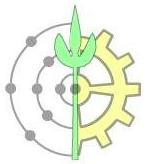
\includegraphics{Logo} %%% insere a imagem
\end{lstlisting}
\end{tcolorbox}
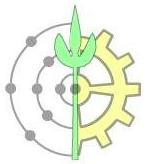
\includegraphics{Logo}

A classe estilo procura as imagens primeiro em uma pasta chamada "\textsf{Imagens}"\, que deve estar no mesmo diretório de seu arquivo tex, se essa pasta não existir a imagem será procurada na mesma pasta do arquivo tex, se o arquivo não existir a compilação falhará e será exibida a mensagem de erro: \textit{File not found}.

O comando \verb|includegraphics{arquivo}| apenas insere a imagem, para que tenha legenda é necessário colocá-la dentro de um ambiente \verb|figure|, onde também é possível controlar seu posicionamento horizontal.
\begin{tcolorbox}
\begin{lstlisting}
\begin{figure}[H]
    \centering %%% Centraliza a imagem
    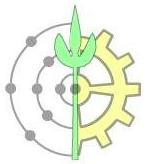
\includegraphics{Logo} %%% Insere a imagem
    \caption{Este é o logotipo da UFRRJ} %%% Legenda da imagem
    \label{Logorural} %%% Marca para fazer referência cruzada
\end{figure}
\end{lstlisting}
\end{tcolorbox}
\begin{figure}[H]
	\centering %%% centraliza a imagem
	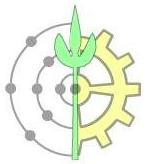
\includegraphics{Logo}
	\caption{Este é o logotipo da UFRRJ} %%% legenda da imagem
	\label{Logorural} %%% Marca para fazer referência cruzada
\end{figure}


\begin{tcolorbox}
\begin{lstlisting}
\begin{figure}[H]
   \centering
   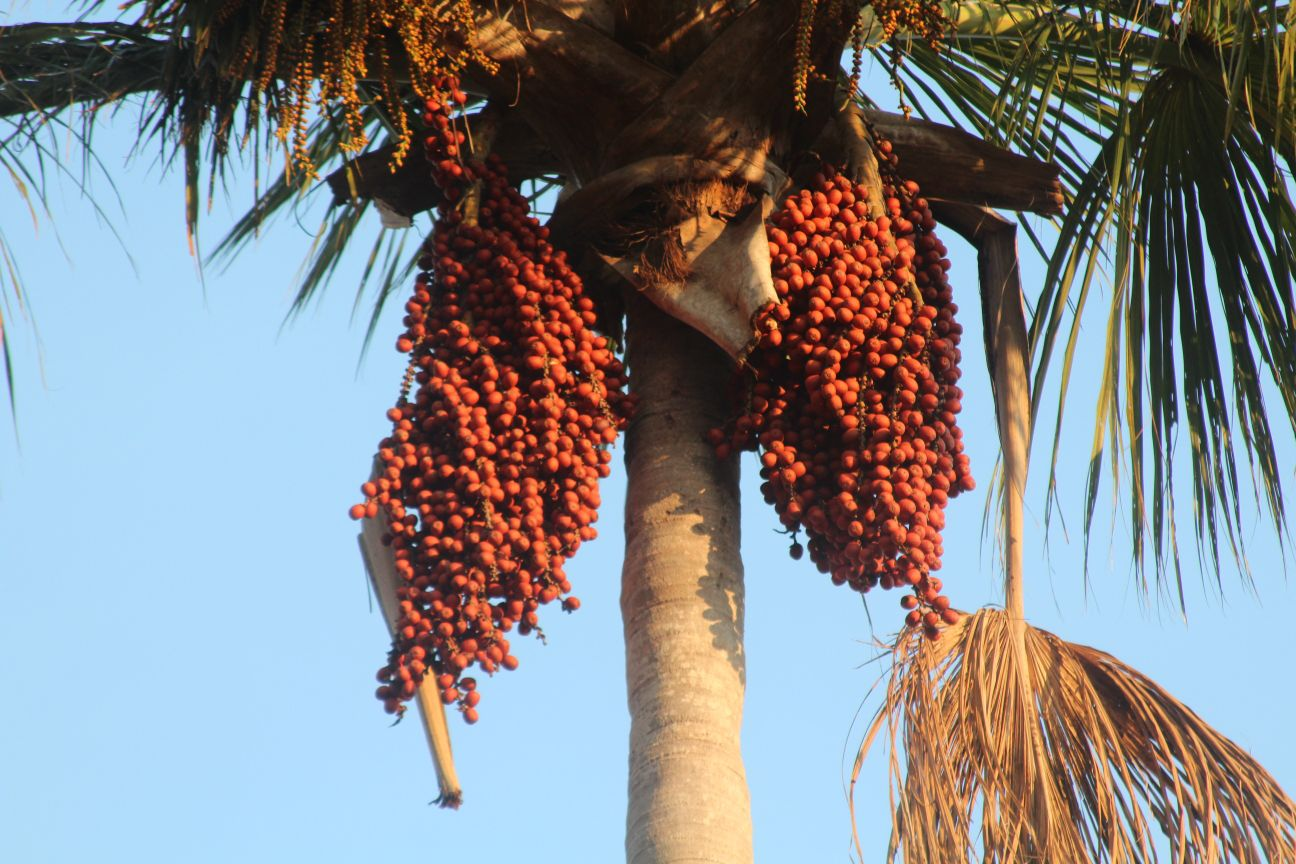
\includegraphics[scale=0.15]{Buriti}
   \caption{Imagem reduzia a $15\%$ do seu tamanho}
\end{figure}
\end{lstlisting}
\end{tcolorbox}
\begin{figure}[H]
   \centering
   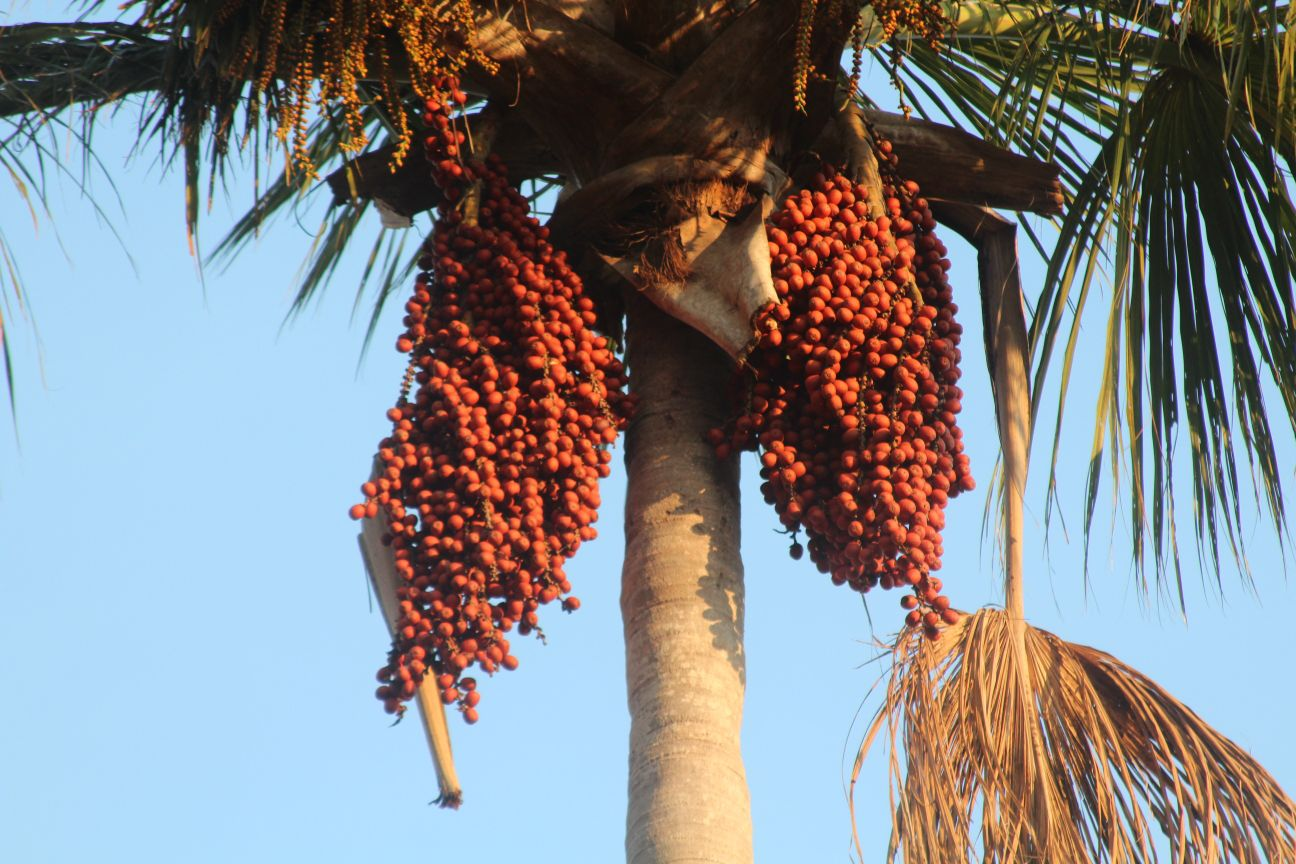
\includegraphics[scale=0.15]{Buriti}
   \caption{Imagem reduzia a $15\%$ do seu tamanho}
   \label{primeira}
\end{figure}

Uma opção muito comum ao lidar com imagem consiste em ajustar seu tamanho para coincidir com a largura da página, o comando \verb|\resizebox| faz esse ajuste
\begin{tcolorbox}
\begin{lstlisting}
\begin{figure}[H]
   \resizebox{\textwidth}{!}{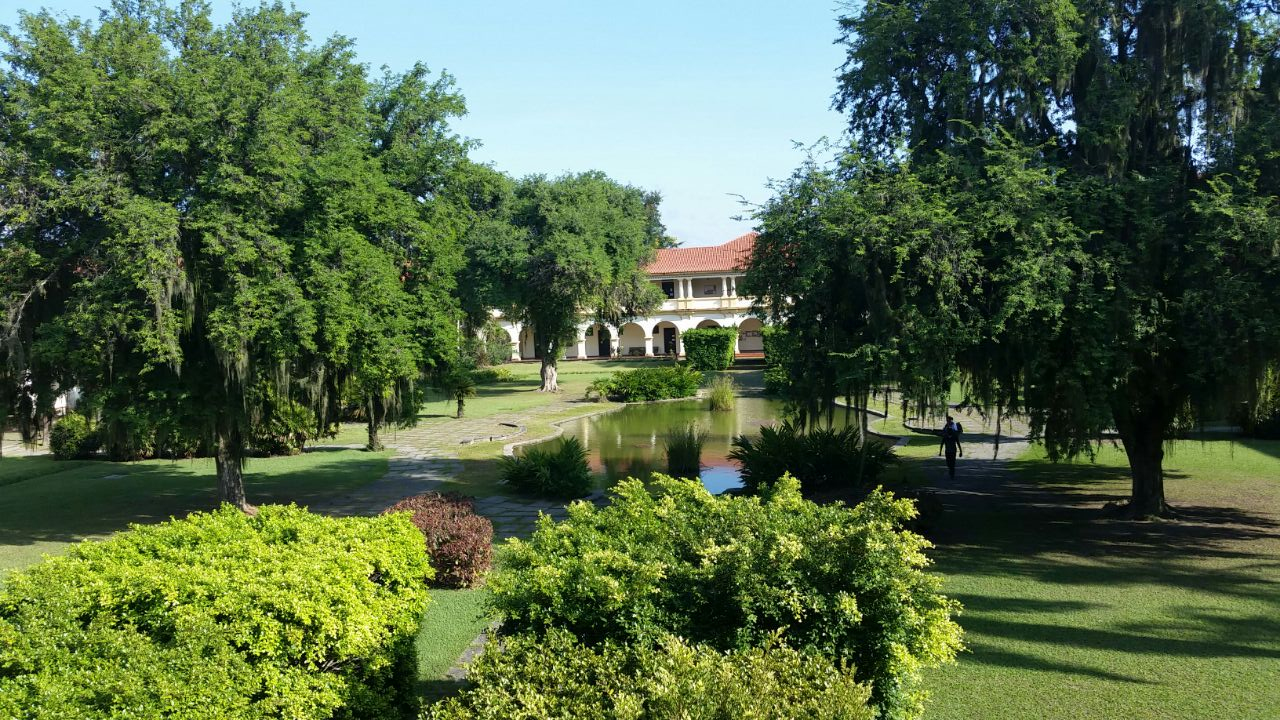
\includegraphics{RuralP1}}
   \caption{O prédio principal da UFRRJ, vulgo P1}
   \label{op1} %%% Marca para referência cruzada
\end{figure}
\end{lstlisting}
\end{tcolorbox}
\begin{figure}[H]
	\resizebox{\textwidth}{!}{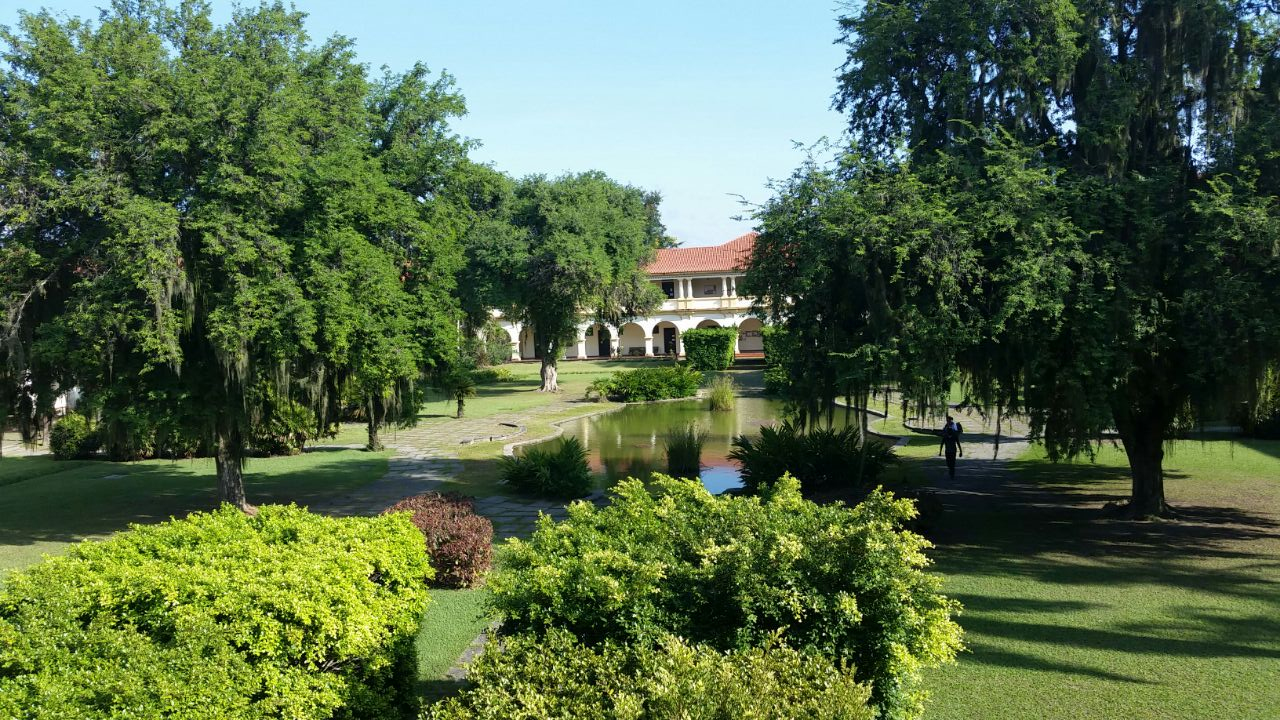
\includegraphics{RuralP1}}
	\caption{O prédio principal da UFRRJ, vulgo P1}
	\label{op1}
\end{figure}

\subsection{Girando de imagem}

É muito simples girar uma imagem no sentido horário ou anti-horário.
\begin{tcolorbox}
\begin{lstlisting}
\begin{figure}[H]
   \centering
   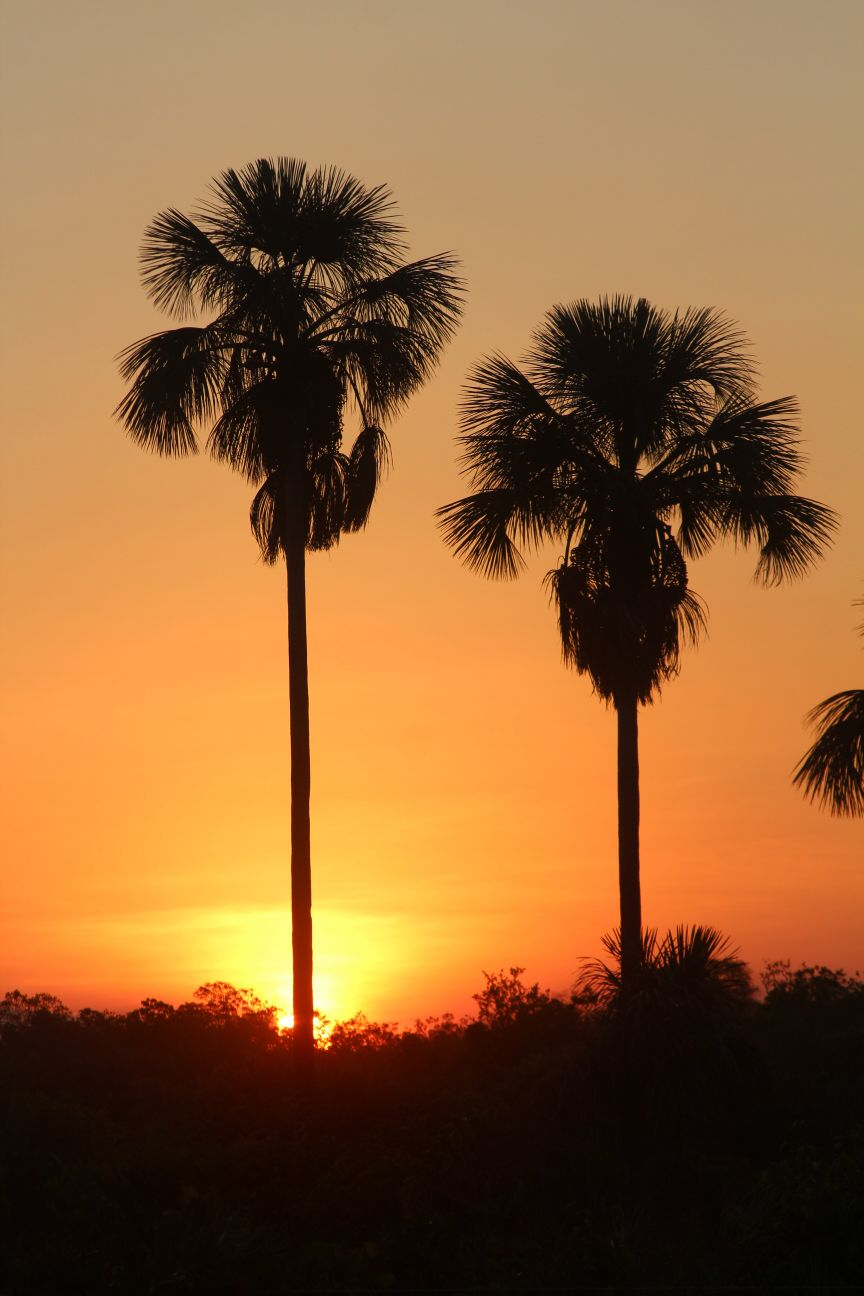
\includegraphics[scale=0.1,angle=-15]{Buritis}
   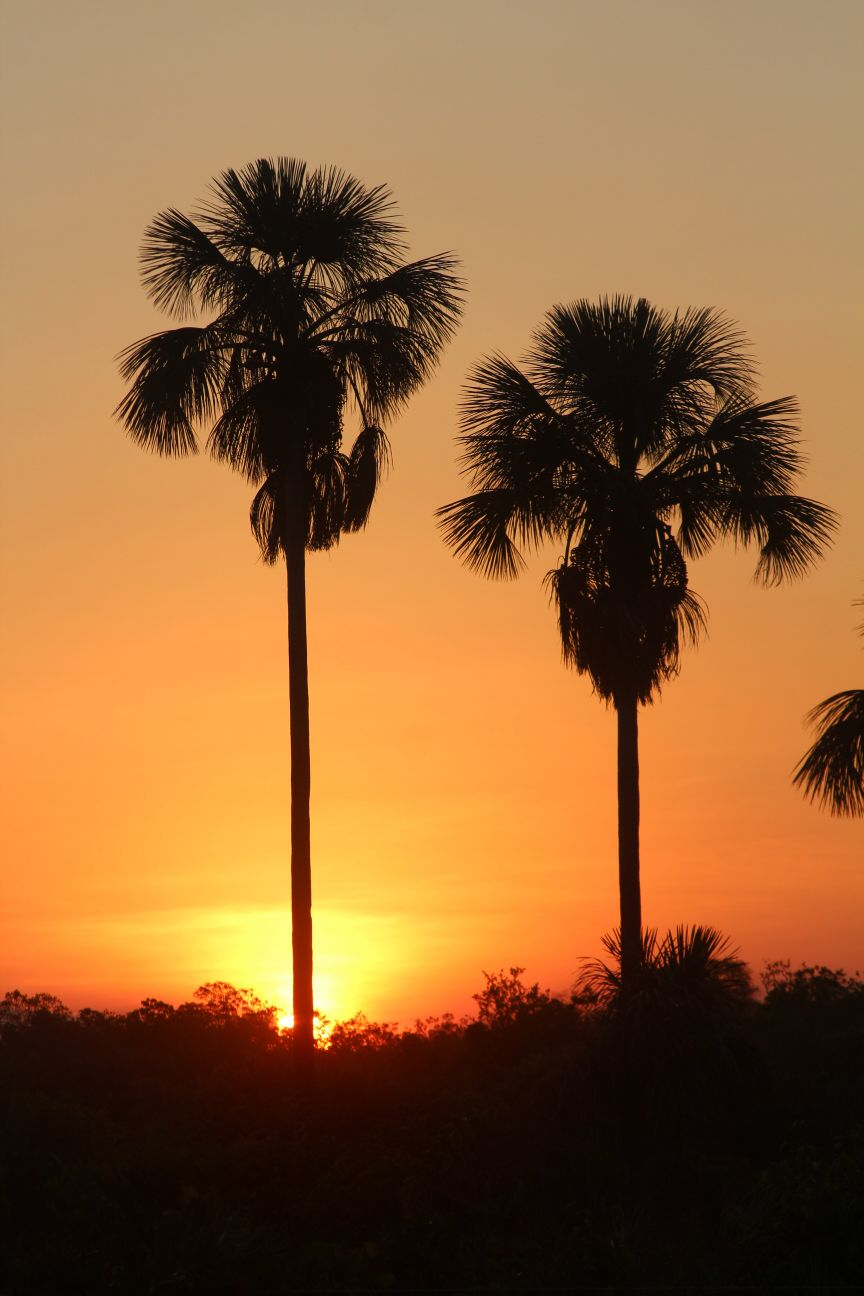
\includegraphics[scale=0.1]{Buritis}
   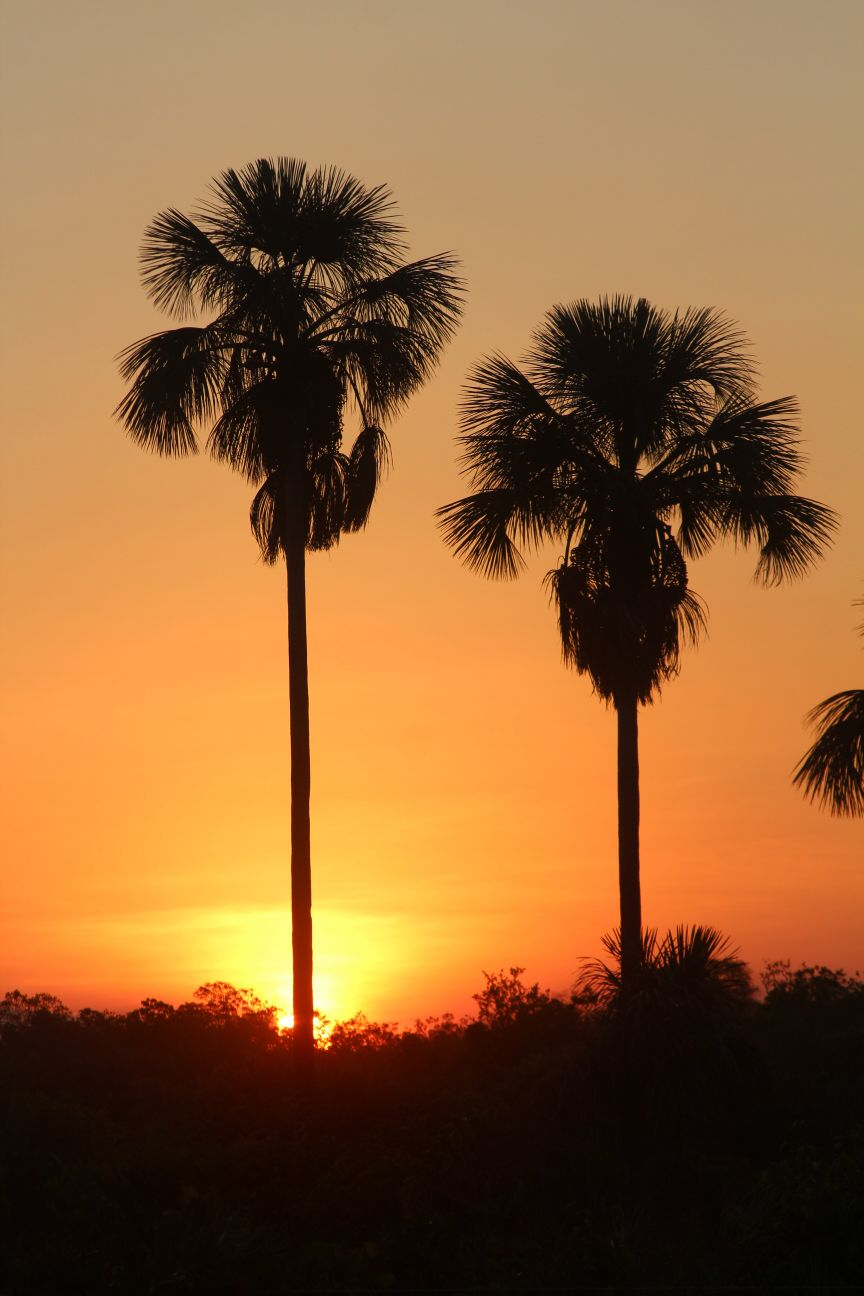
\includegraphics[scale=0.1,angle=15]{Buritis}
   \caption{Girando imagens}\label{giraas}
\end{figure}
\end{lstlisting}
\end{tcolorbox}

\begin{figure}[H]
	\centering
	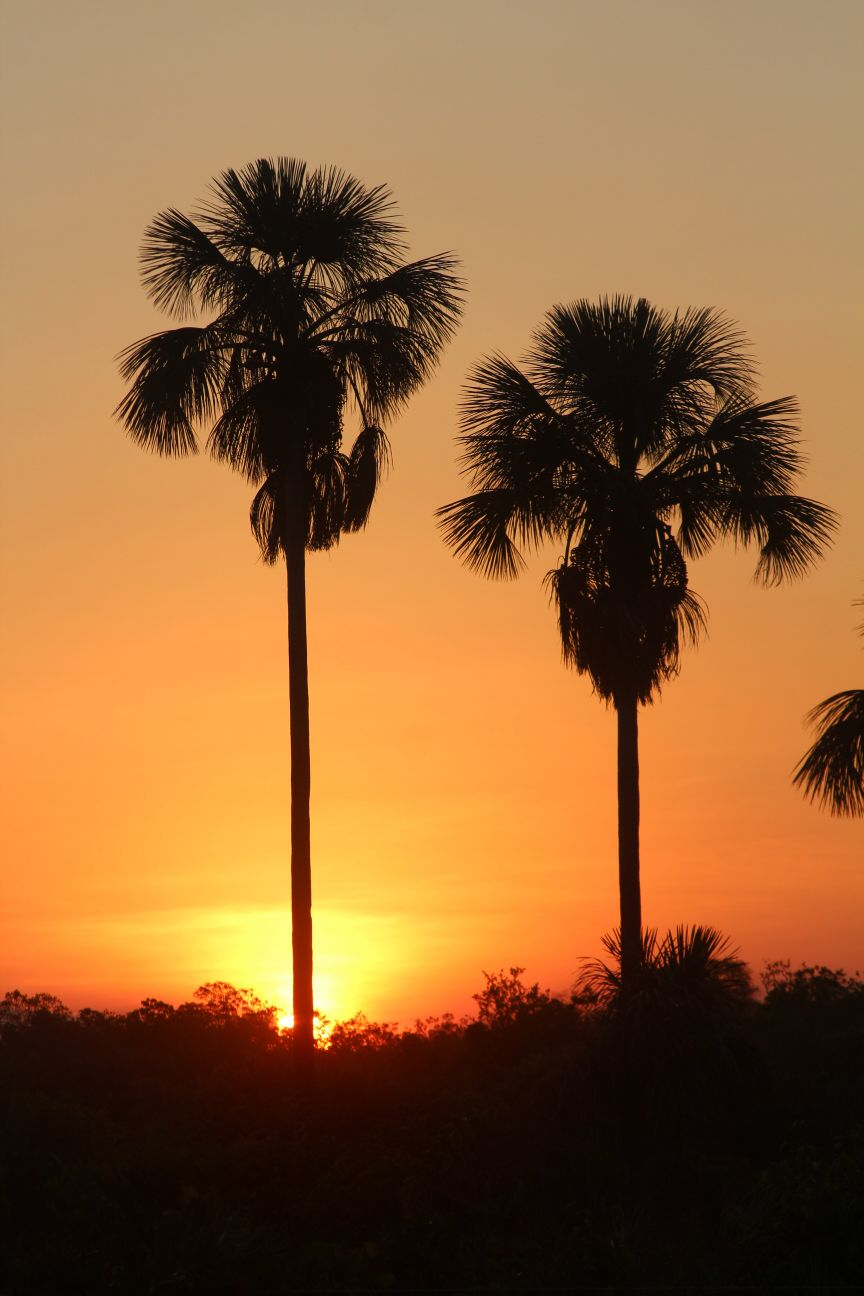
\includegraphics[scale=0.1,angle=-15]{Buritis}
	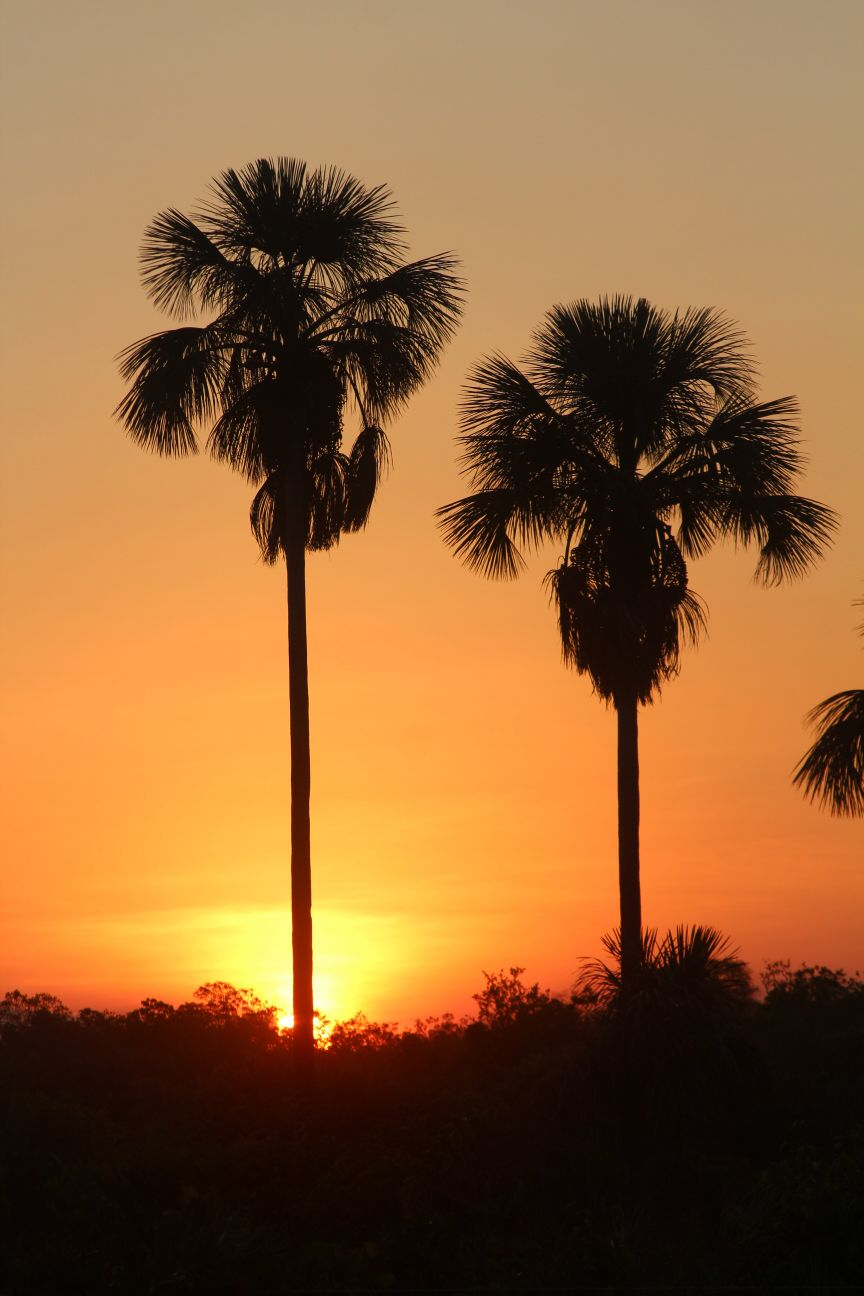
\includegraphics[scale=0.1]{Buritis}
	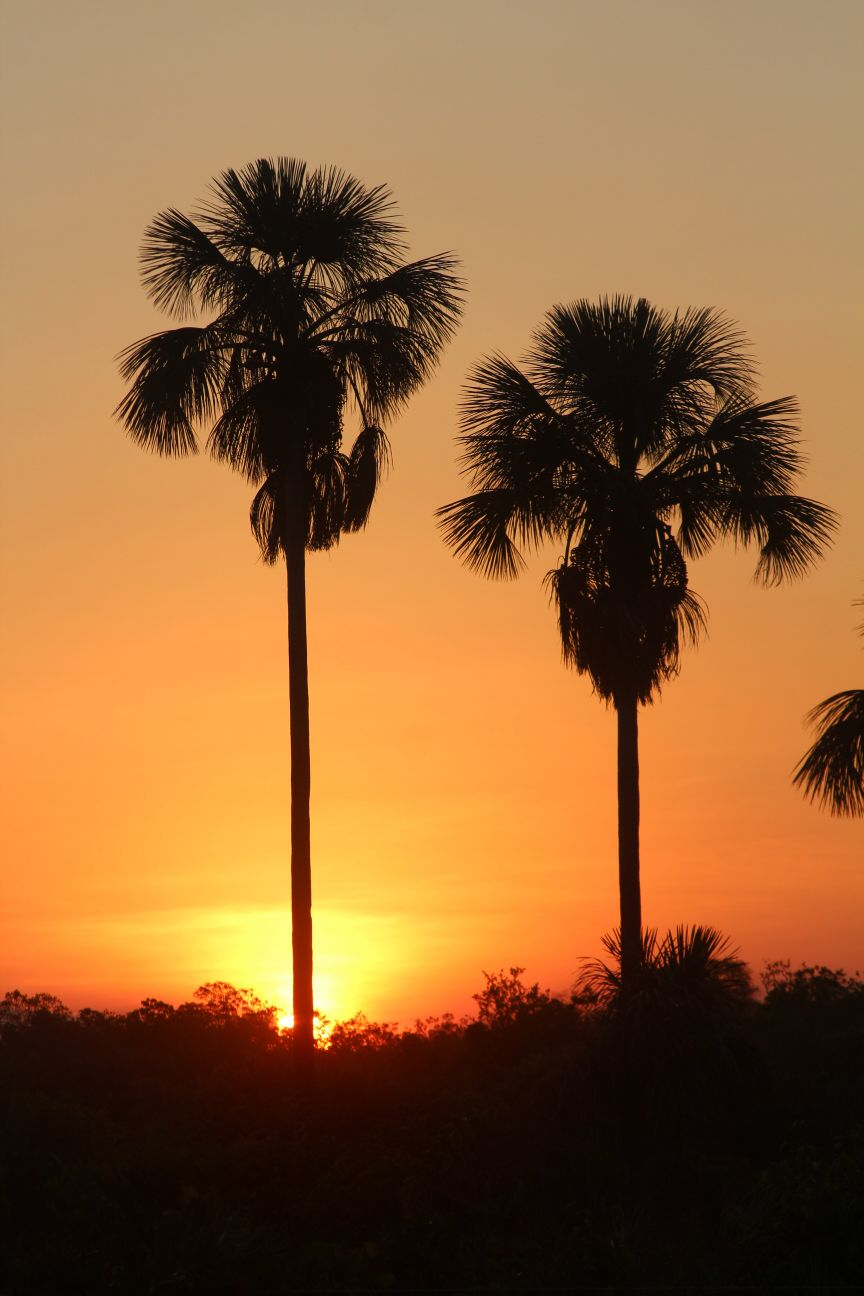
\includegraphics[scale=0.1,angle=15]{Buritis}
	\caption{Girando imagens}\label{giraas}
\end{figure}


\subsection{Imagens lado a lado}

\begin{tcolorbox}
\begin{lstlisting}
\begin{figure}[H]
   \centering
   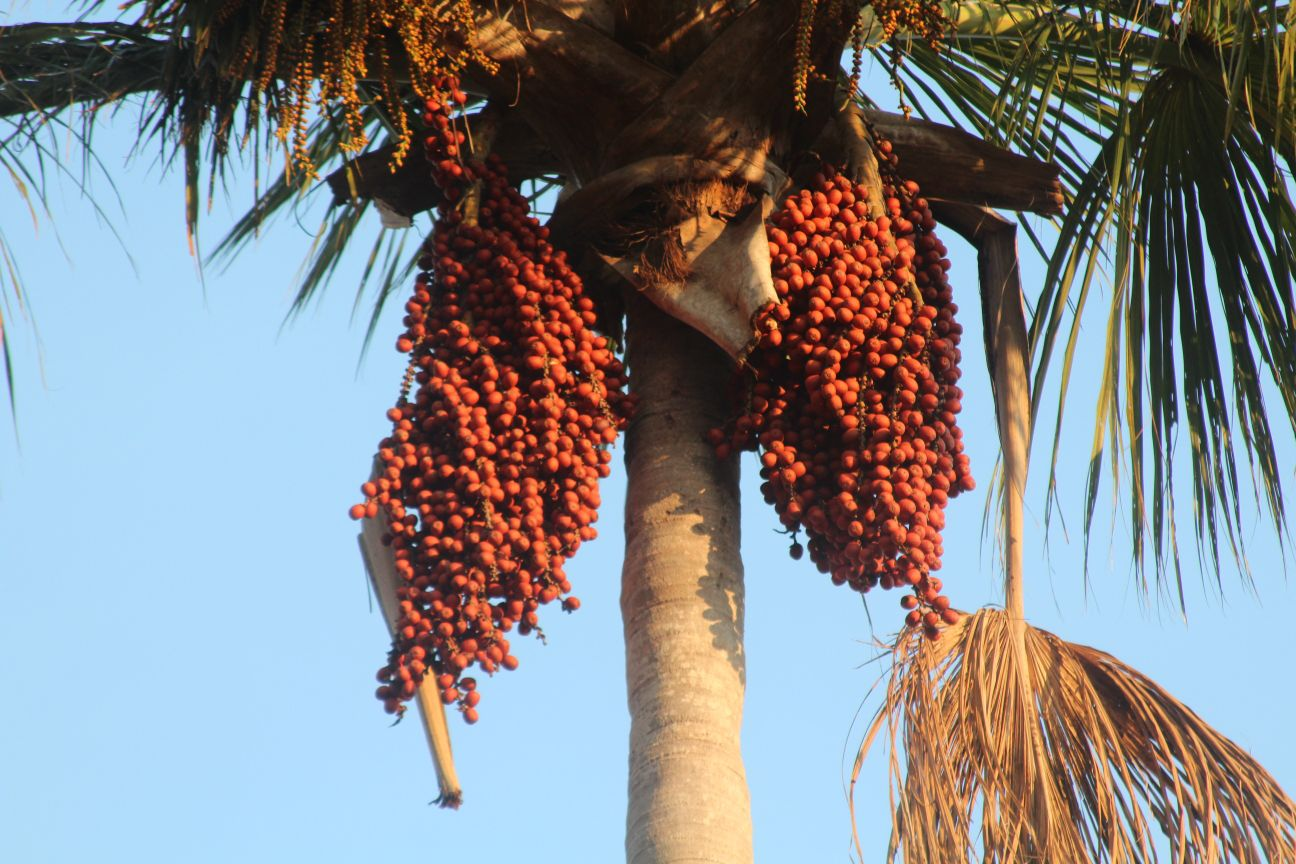
\includegraphics[scale=0.1]{Buriti}
   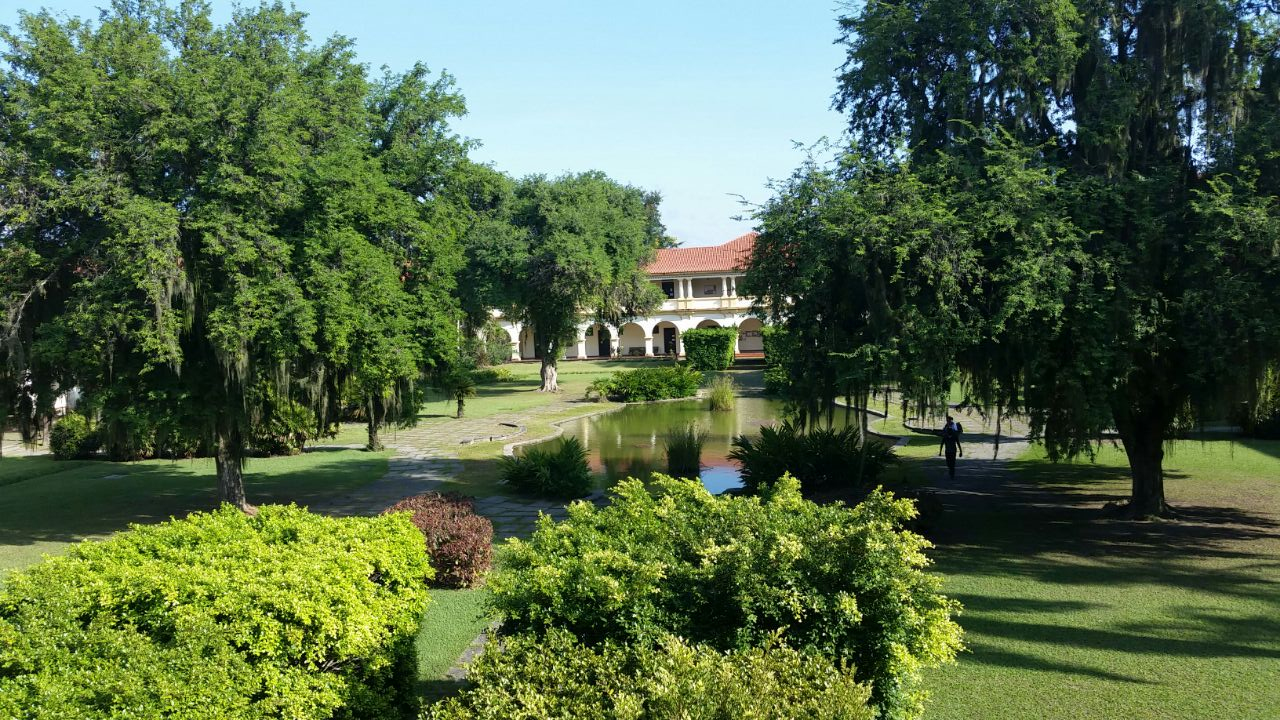
\includegraphics[scale=0.1]{RuralP1}
   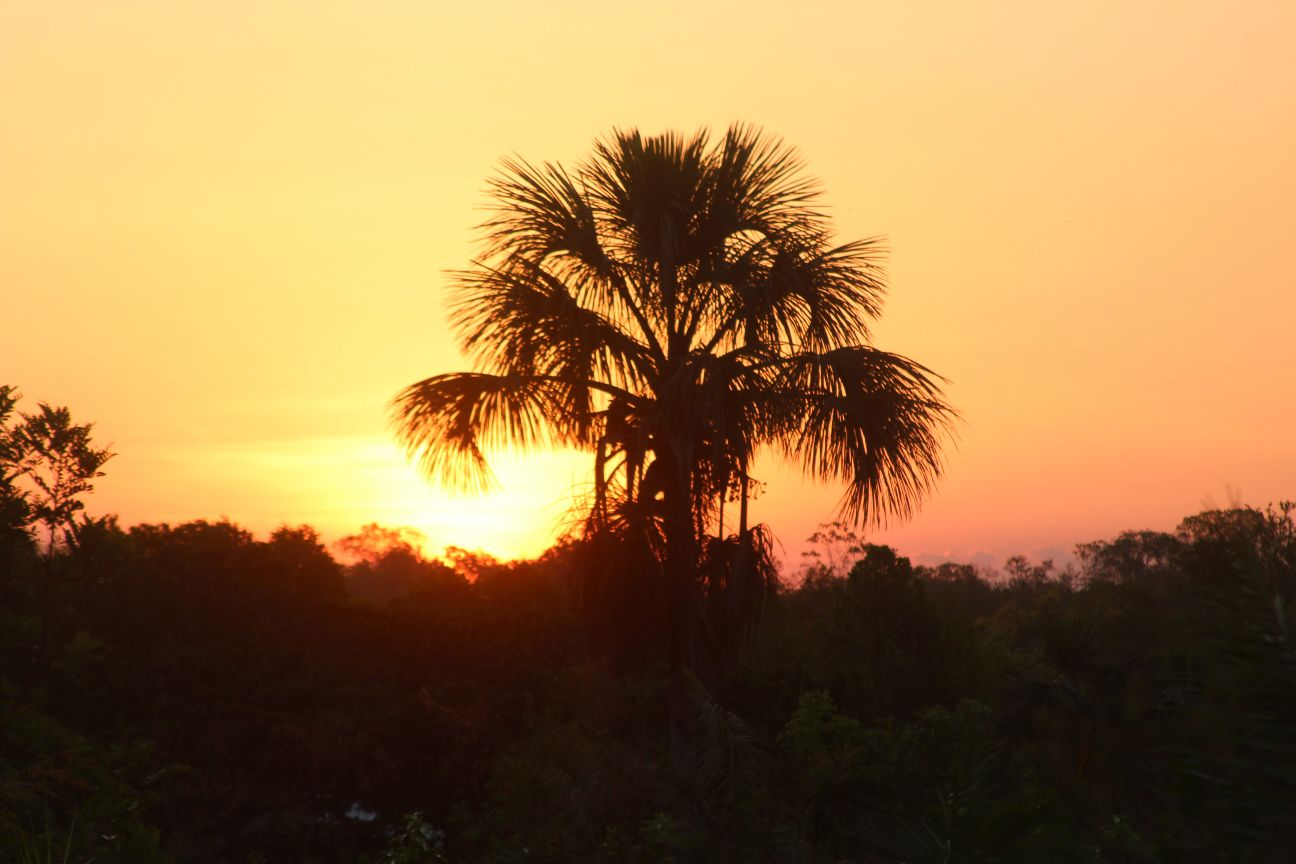
\includegraphics[scale=0.1]{Pordosol}
   \caption{Imagens lado a lado}\label{ladoalado}
\end{figure}
\end{lstlisting}
\end{tcolorbox}

\begin{figure}[H]
	\centering
	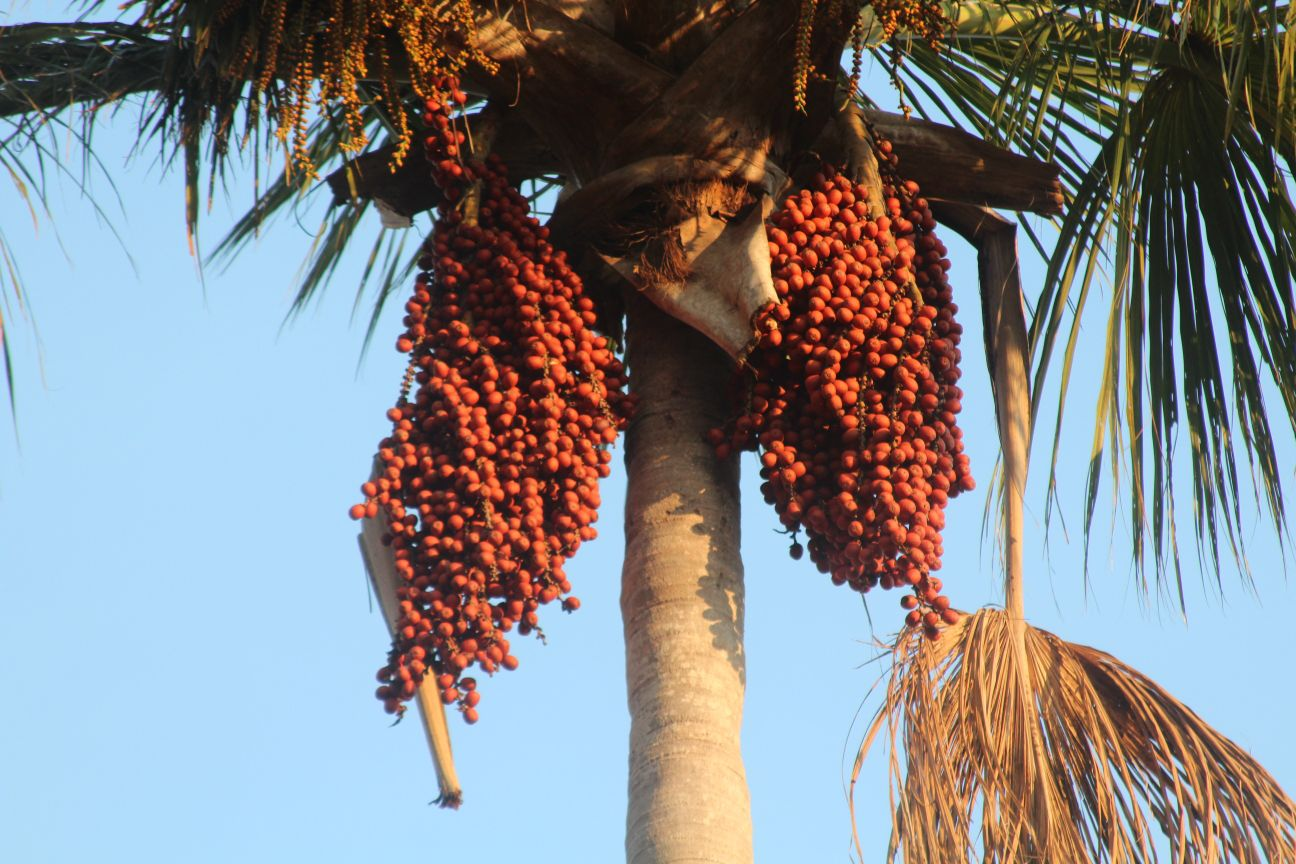
\includegraphics[scale=0.1]{Buriti}
	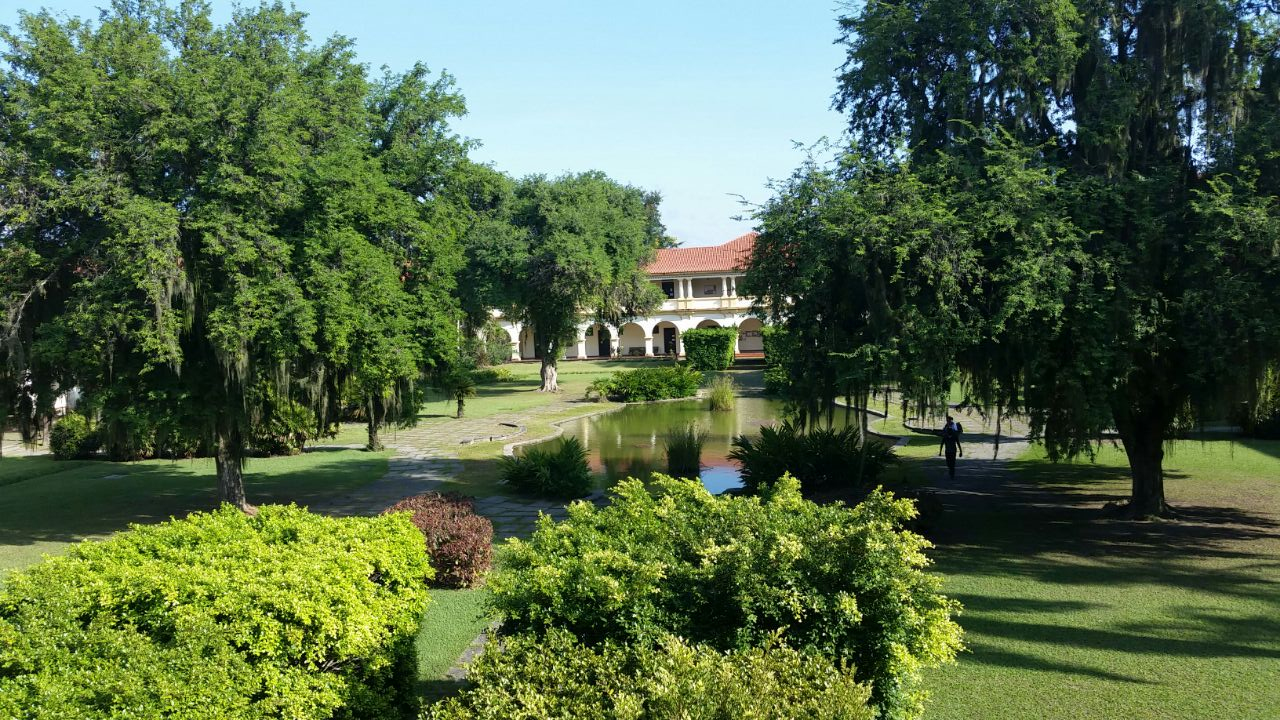
\includegraphics[scale=0.1]{RuralP1}
	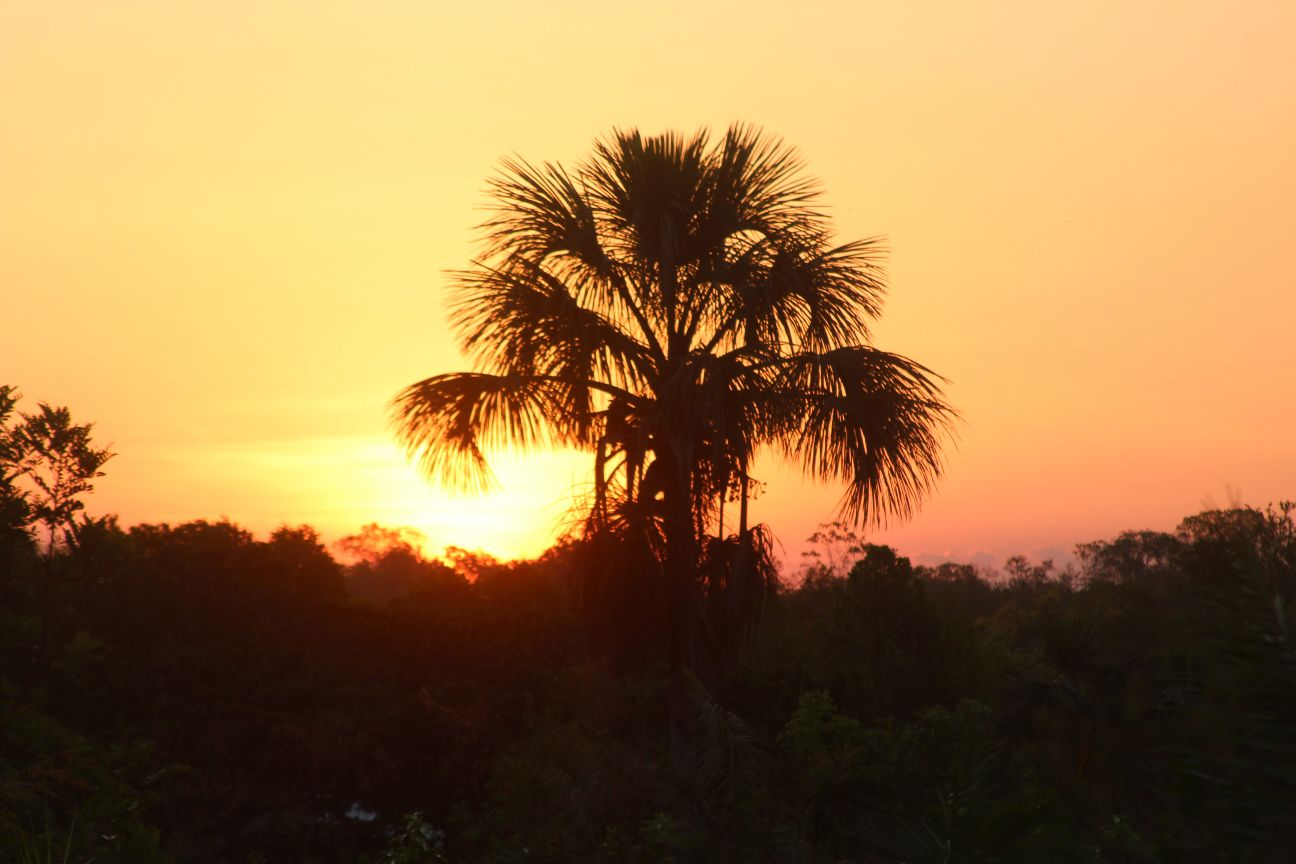
\includegraphics[scale=0.1]{Pordosol}
	\caption{Imagens lado a lado}\label{ladoalado}
\end{figure}

Para inserir uma legenda para cada figura e uma legenda geral tem-se a seguinte opção
\begin{tcolorbox}
\begin{lstlisting}
\begin{figure}[H]
   \centering
   \subcaptionbox{Fruta do buriti \label{fruta}}[0.33\linewidth]{%
		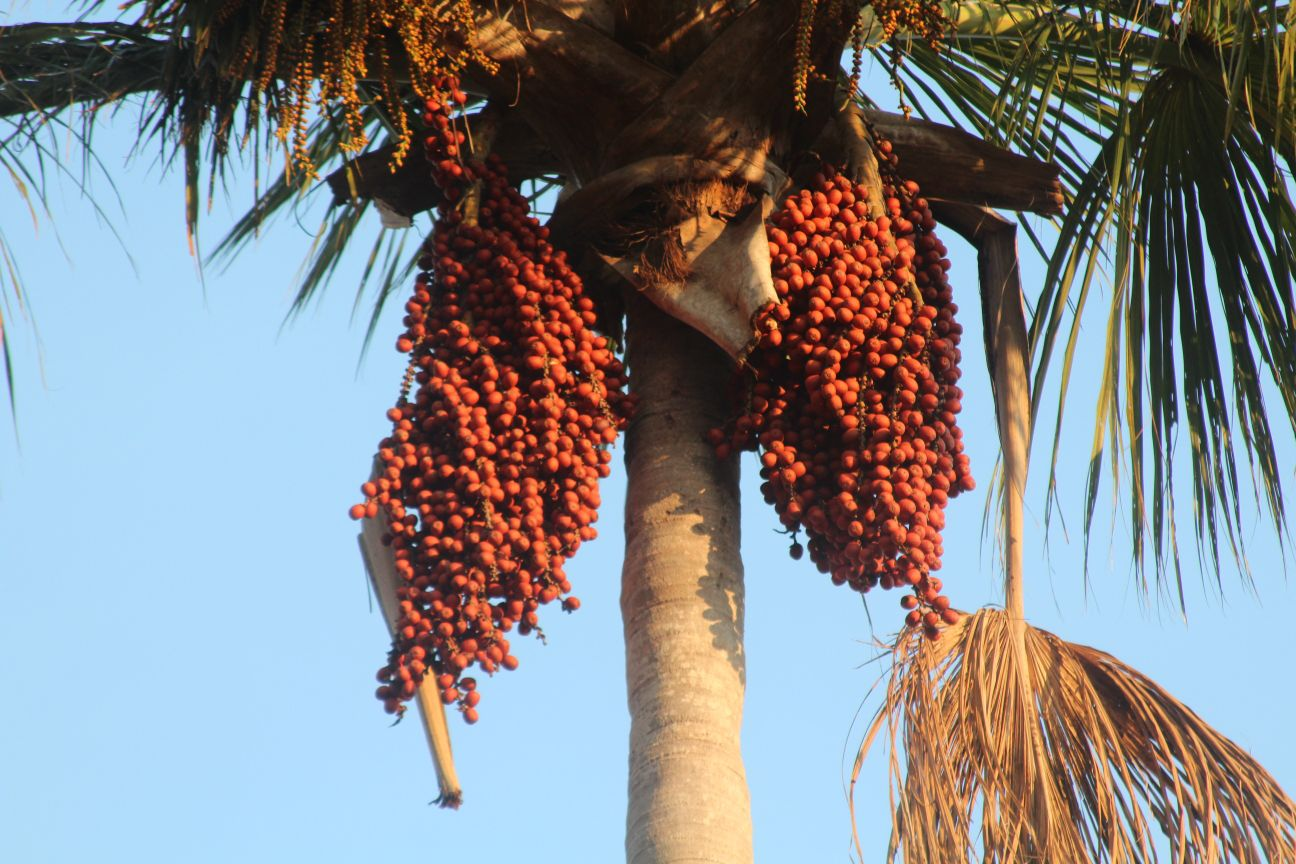
\includegraphics[scale=0.1]{Buriti}} %
   \subcaptionbox{Bonito por do sol e uma sublegenda intencionalmente
        grande\label{Pordosol}}[0.33\linewidth]{%%%
        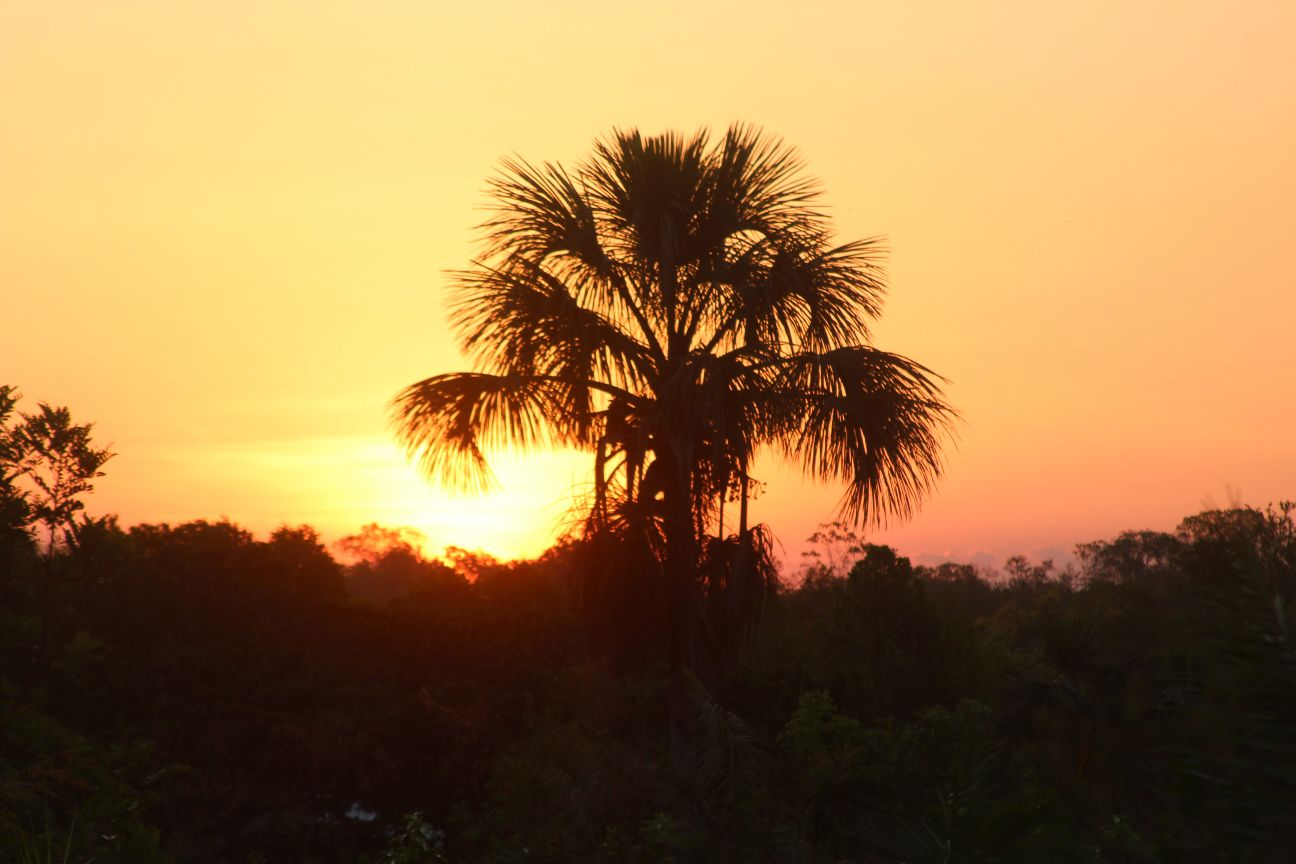
\includegraphics[scale=0.1]{Pordosol}}
   \subcaptionbox {Duas palmeiras de buriti \label{duas}}[%%%
        0.3\linewidth]{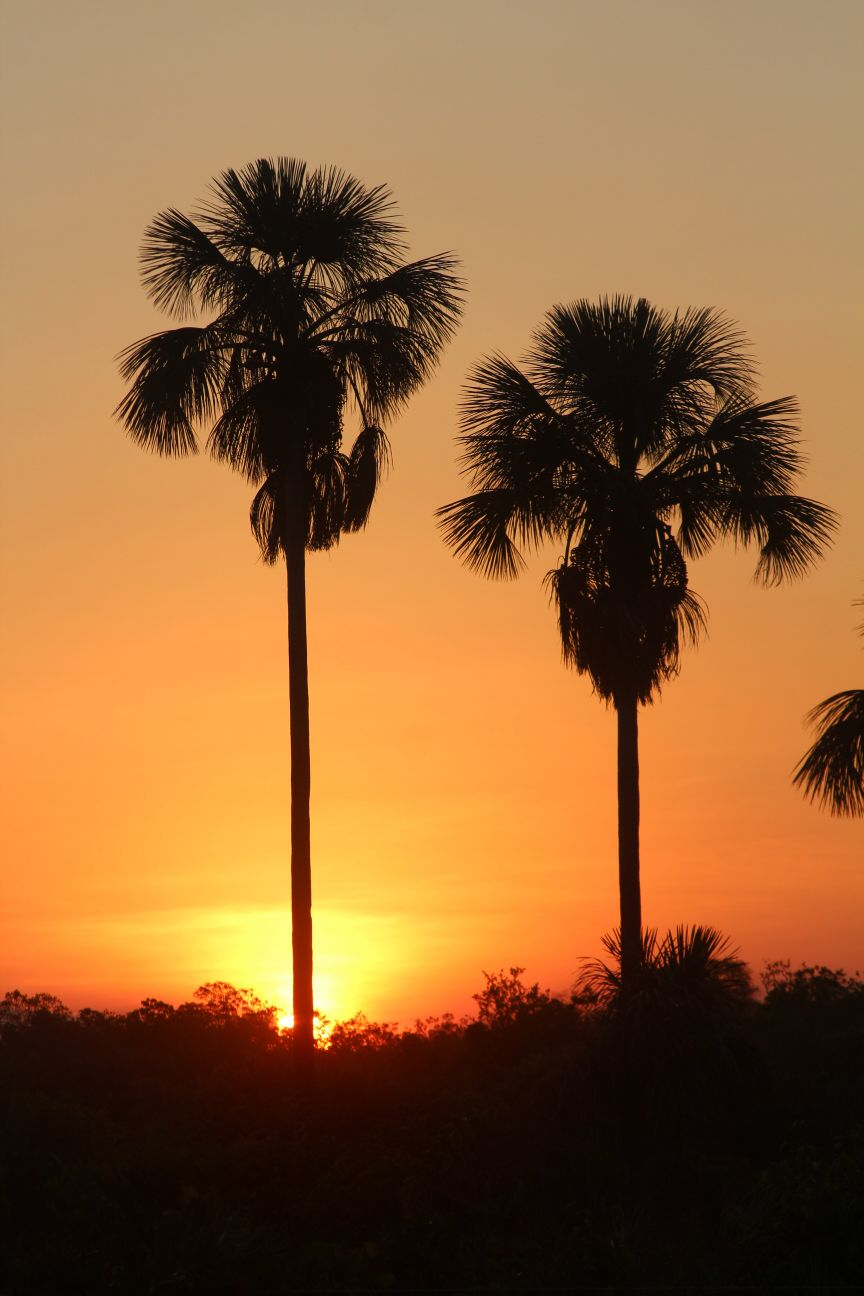
\includegraphics[scale=0.12]{Buritis}} %
   \caption{Buriti é uma palmeira de fruto saboroso}\label{buritis}
\end{figure}
\end{lstlisting}
\end{tcolorbox}
\begin{figure}[H]
	\centering
	\subcaptionbox{Fruta do buriti \label{fruta}}[0.33\linewidth]{%
		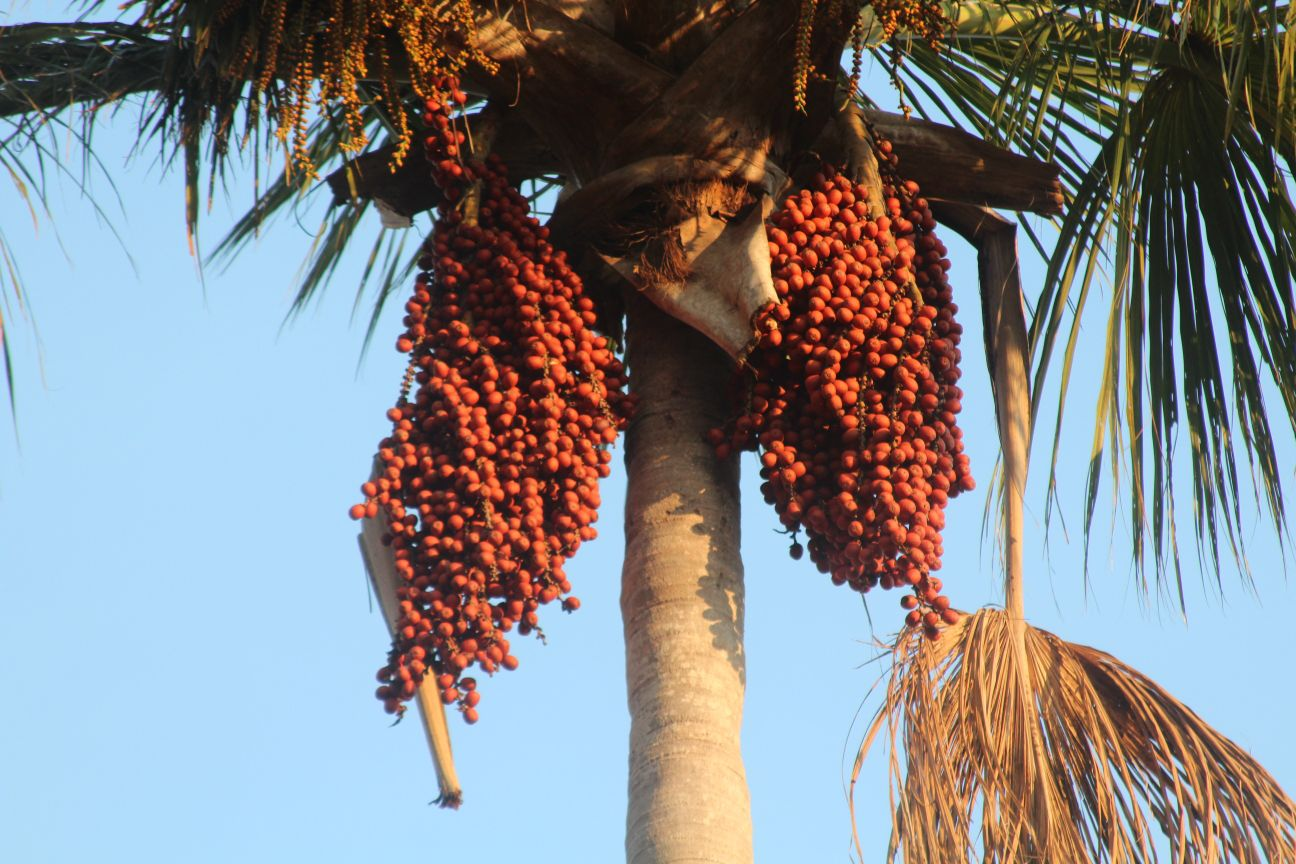
\includegraphics[scale=0.1]{Buriti}} %
	\subcaptionbox{Bonito por do sol e uma sublegenda intencionalmente grande
		\label{Pordosol}}[0.33\linewidth]{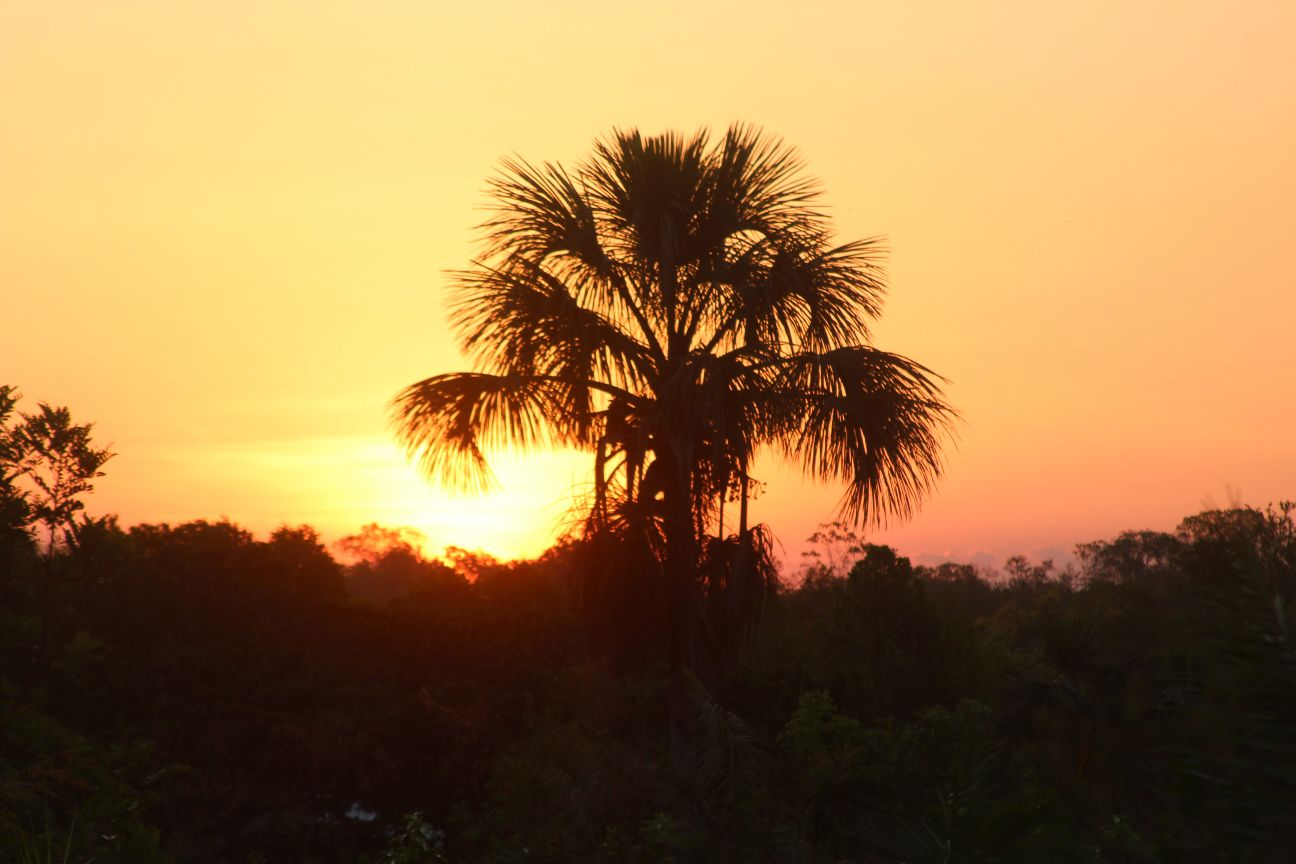
\includegraphics[scale=0.1]{Pordosol}}
	\subcaptionbox {Duas palmeiras de buriti \label{duas}}[0.3\linewidth]{%%%
		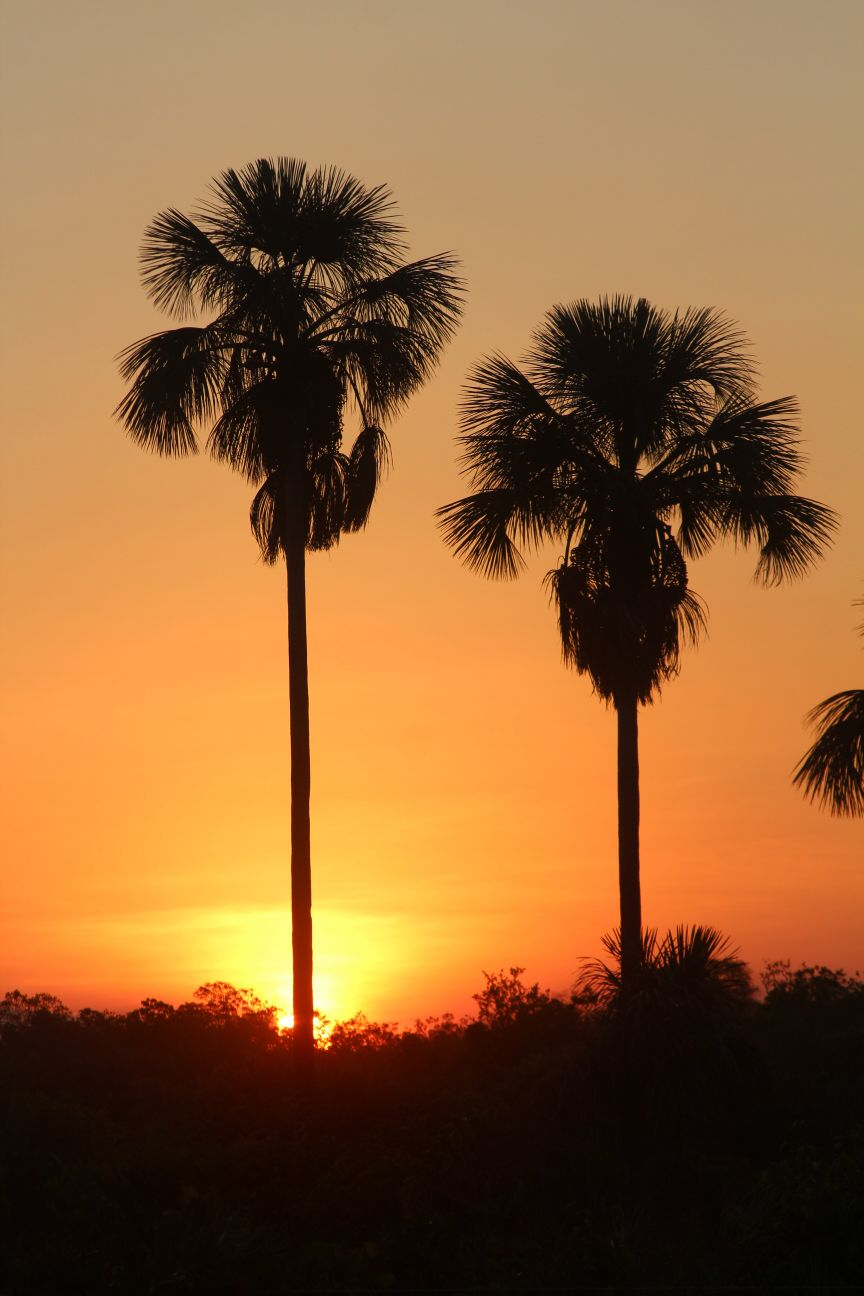
\includegraphics[scale=0.12]{Buritis}} %
	\caption{Buriti é uma palmeira de fruto saboroso}\label{buritis}
\end{figure}


\section{Inclusão de imagem com a classe estilo}

O comando para inserir imagem é o \verb|\includegraphics{imagem}|. 
Alternativamente a classe estilo definiu os comandos: \verb|\imagem| e 
\verb|\imagemlp|. Esses comandos são muito parecidos, o primeiro insere a imagem 
em tamanho natural, o segundo ajusta a largura da imagem à largura da página sem 
provocar distorções, ambos possuem três argumentos, um opcional e dois 
obrigatórios. Veja o manual.


Tanto o \verb|\imagem| quanto o \verb|\imagemlp| inserem a imagem dentro de um ambiente \texttt{table} carregado com o posicionador H, isso implica que a imagem ficará onde foi inserida de qualquer jeito.

Além de seu nome ser mais simples e fácil de manipular, esses dois comandos se encarregam de inserir todos os bons adereços que uma imagem em geral requer, tornando significativamente mais simples a manipulação de imagem.

A imagem~\ref{primeira} foi inserida com o código
\begin{tcolorbox}
\begin{lstlisting}
\begin{figure}[H]
   \centering
   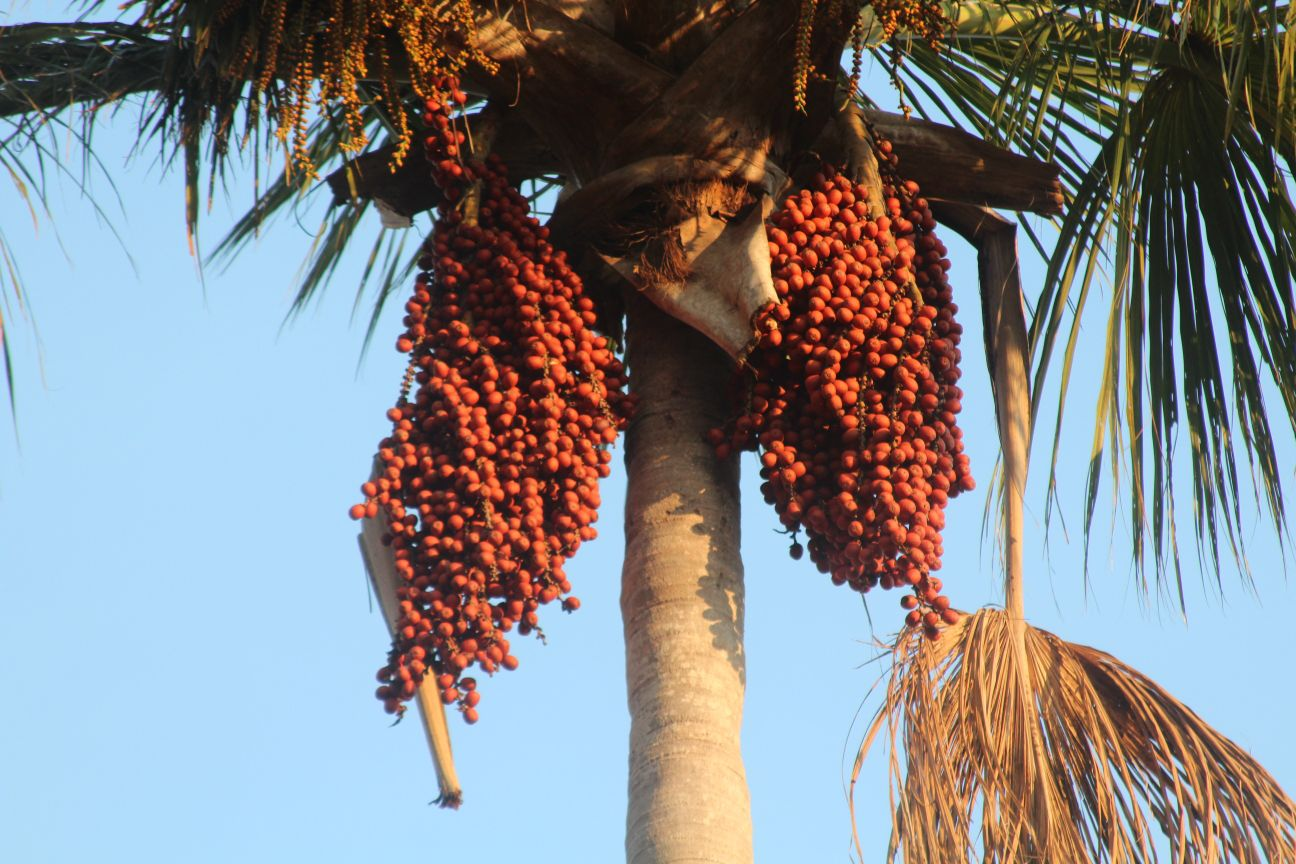
\includegraphics[scale=0.15]{Buriti}
   \caption{Imagem reduzia a $15\%$ do seu tamanho}
\end{figure}
\end{lstlisting}
\end{tcolorbox}

O mesmo resultado é obtido com o singelo fragmento
\begin{tcolorbox}
\begin{lstlisting}
\imagem[scale=0.15]{Buriti}{Imagem reduzia a $15\%$ do seu tamanho}
\end{lstlisting}
\end{tcolorbox}
\imagem[scale=0.15]{Buriti}{Imagem reduzia a $15\%$ do seu tamanho}

Da mesma forma, a imagem~\ref{op1} foi inserida com o código
\begin{tcolorbox}
\begin{lstlisting}
\begin{figure}[H]
   \resizebox{\textwidth}{!}{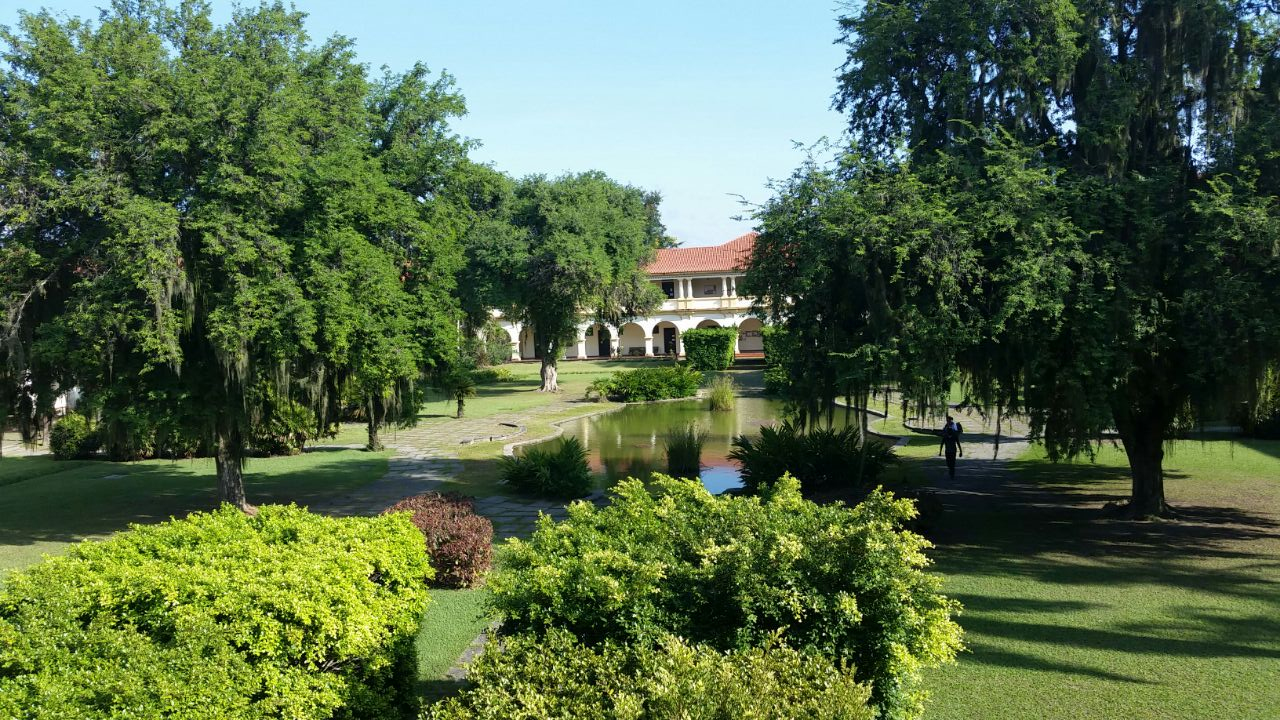
\includegraphics{RuralP1}}
   \caption{O prédio principal da UFRRJ, vulgo P1}
   \label{op1} %%% Marca para referência cruzada
\end{figure}
\end{lstlisting}
\end{tcolorbox}

O mesmo resultado é obtido com o código
\begin{tcolorbox}
\begin{lstlisting}
\imagemlp{RuralP1}{O prédio principal da UFRRJ, vulgo P1}
\end{lstlisting}
\end{tcolorbox}
\imagemlp{RuralP1}{O prédio principal da UFRRJ, vulgo P1}


\begin{tcolorbox}
\begin{lstlisting}
   Note que a imagem~\ref{RuralP1} foi ajustada para a largura da página, enquanto a imagem~\ref{Buriti}, por meio do argumento opcional $scale=0.15$, teve seu tamanho reduzido a $15\%$.
\end{lstlisting}
\tcblower
Note que a imagem~\ref{RuralP1} foi ajustada para a largura da página, enquanto a imagem~\ref{Buriti}, por meio do argumento opcional $scale=0.15$, teve seu tamanho reduzido a $15\%$.
\end{tcolorbox}

Observe como a referência cruzada foi feita utilizando o próprio nome do arquivo da imagem, sem necessidade de incluir o \verb|\label{RuralP1}| e \verb|\label{Buriti}|, essa é uma vantagem de usar os comandos da classe estilo.

\imagem{Esquema}{Imagem em pdf}
\chapter{Códigos}\label{codigos}

Há duas formas para inserir um código, ambas exigem que seja carregada a 
opção de classe ``codigo''. Carregada essa opção ficam disponíveis as 
ferramentas do pacote \texttt{listings}, as duas principais são exemplificadas 
a seguir.

\section{Inserindo o código de um arquivo}

Essa possibilidade não admite os acentos ortográficos da língua portuguesa, 
mesmo que estejam em comentário. Mas se o código for copiado para o arquivo tex
os acentos não serão um problema.

Para que o \LaTeX\ dê o devido tratamento ao conteúdo do arquivo 
deve-se informar a qual linguagem o código pertence. São aceitas 
muitas linguagens e alguns dialetos de linguagens, para ver a 
lista completa veja o manual do pacote \pacote{listings}.
Algumas exemplos:

Para inserir código do Matlab use \epar{language}{Matlab}

Para inserir código do Maple use \epar{language}{Maple}.

Para inserir código do C use \epar{language}{C}.

Para inserir código do C++ use \epar{language}{C++}.

Para inserir código do Java use \epar{language}{Java}.

Para inserir código do Fortran use \epar{language}{Fortran}.

Para inserir código do Python use \epar{language}{Python}.

Para inserir código do Pascal use \epar{language}{Pascal}.

Para inserir código do Octave use \epar{language}{Octave}.

No exemplo a seguir foi utilizado um código do matlab, por isso
foi inserida a chave \epar{language}{Matlab} para dizer ao \LaTeX\
que o conteúdo do arquivo Laplace.m é um código do MatLab.

\begin{tcolorbox}[breakable]
\begin{lstlisting}
   \lstinputlisting[language=Matlab,captionpos=b]{Laplace.m}
\end{lstlisting}
\tcblower
\lstinputlisting[language=Matlab,captionpos=b]{Laplace.m}
\end{tcolorbox}

\section{Inserindo o código diretamente}

Para inserir um código basta colocá-lo dentro do ambiente \textsf{lstlisting}. Sua sintaxe é:
\begin{center}
	\begin{minipage}{0.7\textwidth}
		\azul{\coma{begin}}$\{$\verde{\textsf{lstlisting}}$\}$[\op{opções}]
		
		\vspace{0.2cm}
		\hspace{0.5cm}\textit{Conteúdo do ambiente, o código.}
		\vspace{0.2cm}
		
		\azul{\coma{end}}$\{$\textsf{\verde{lstlisting}}$\}$
	\end{minipage}
\end{center}

\begin{tcolorbox}[breakable,title={Código posto dentro de um ambiente lstlisting}]
\begin{lstlisting}[language=Matlab,
caption={Exemplo de inclusão de código},captionpos=b]
m = input('Digite o numero de linhas ');
n = input('Digite o numero de colunas ');
%%% Montando a Matriz do sistema Bloco diagonal
A = zeros(n,m);
nl1 = n - 1;  np1 = n + 1;
msize = n*m;  msln = msize - n;
%%% As três diagonais: Diagonal principal, acima e abaixo
A(1,1) = -4.0; %%% Primeiro valor da diagonal principal
for i = 2:msize
   A(i-1,i) = 1.0;  %%% Abaixo
   A(i,i)   =-4.0;  %%% Valores da diagonal principal
   A(i,i-1) = 1.0;  %%% Acima
end
% Correção: Substituindo alguns valores 1 por 0
for i = n:n:msln
   A(i,i+1) = 0.0;
   A(i+1,i) = 0.0;
end
%%% Diagonais afastadas
for i = np1:msize
   A(i,i-n) = 1.0;
   A(i-n,i) = 1.0;
end
%%% Lado direito do sistema (inclui os valores de fronteira)
b=zeros(msize,1);
%%% Atualiza os valores não nulos
for i = n:n:msize
   b(i,1) = -100;
end
u = A\b % Solução do sistema linear.
% Ordenamento matricial dos valores da temperatura
k = 0;
for i = 1:m
   for j = 1:n
      k = k + 1;
      Temp(i,j) = u(k);
   end
end
Temp
\end{lstlisting}

\end{tcolorbox}






\chapter{Elementos Pós-Textuais}

\section{Índice Remissivo}

Pode ser construído de forma eficiente, simples e consistente com
o pacote \pacote{makeidx}. Vários textos descrevem como construir
um Índice Remissivo com este pacote, veja por exemplo,
\ttt{\LaTeX{} tintim por tintim}.

\section{Referências}

Todas as formas de construir referência com o \LaTeX{} são suportadas
pela classe \estilo, mas apenas três estão configuradas em opções de classe.
\begin{itemize}
	\item{\negri refkom}: é o padrão nas classes scrkook e estilo;
	\item{\negri refnum}: sistema de referência numérico, carrega o pacote
	\pacote{natbib};
	\item{\negri refaa}: sistema de referência autor-ano, carrega o pacote
	\pacote{natbib}.
\end{itemize}

Os comandos
\begin{tcolorbox}
\begin{lstlisting}
   \renewcommand{\bibname}{Referências}
   \bibliographystyle{unsrtnat}
   \bibliography{bibliografia}
\end{lstlisting}
\end{tcolorbox}
devem ser inseridos onde a lista de referências deve ser criada.
\begin{itemize}
\item O \cmc{renewcommand}{\coma{bibname}}$\{$Referências$\}$ define o
   título das referências. Sem esse comando o pacote babel traduzirá
   o título para Referências Bibliográficas, termo que ficou obsoleto
   por que atualmente existem referências que não são bibliográficas.
\item \cmc{bibliographystyle}{unsrtnat}: define o estilo de bibliografia, nesse 
caso o \textsf{unsrtnat} que pertence ao pacote natbib, mas você pode escolher 
outros que também atenda as normas.
\item \cmc{bibliography}{bibliografia}: carrega o arquivo
   bibliografia.bib, o banco de referências, o qual deve ficar
   na mesma pasta de seu arquivo .tex e deve ser feito segundo
   as regras do bibtex ou biber. Segue um exemplo mínimo de
   arquivo .bib segundo as regras do bib\TeX.
\end{itemize}

\begin{tcolorbox}[title={Exemplo de arquivo .bib}]
\begin{lstlisting}
@BOOK{casaliorio,
author = "Júnior, R. I.; Iório, V. M.;",
title = "Equações Diferenciais Parciais: Uma introdução",
edition = "2",
address = "Rio de Janeiro",
publisher = "IMPA",
year = "2010",
}
@book{Elon,
author       = {Elon Lages Lima},
title        = {Curso de An\'alise Volume 1},
address      = {Rio de Janeiro, Rio de Janeiro},
publisher    = {IMPA - Projeto Euclives},
edition      = {$11^a$},
isbn         = {85-244-0118-4},
year         = {2004},
}
@BOOK{briggs,
author = "Briggs, Willian L.;",
title = "A Multigrid Tutorial",
edition = "2",
address = "Philadelphia",
publisher = "SIAM",
year = "1987",
}
@ARTICLE{saad,
author = "SAAD, Y.,",
title = {Iterative Methods for Sparse Linear Systems},
journal = {PWS Publish-ing Company},
address = "Boston",
year = 1996,
}
\end{lstlisting}
\end{tcolorbox}

O arquivo .bib que gerou as referências deste manual é distribuído junto com a classe estilo, construa o seu a partir dele acrescentando os seus itens bibliográficos.

A citação é feita com o comando \cmc{cite}{apelido} ou \cmc{citet}{apelido} ou
outros que o pacote natbib oferece, mas apenas o \cmc{cite}{apelido} já é suficiente. O apelido é o primeiro nome do item no seu arquivo .bib. Para fazer referência ao primeiro item do exemplo de arquivo .bib dado deveria ser inserido o comando \cmc{cite}{casaliorio}, veja
\begin{tcolorbox}[title={Sistema de referenciação numérico: opção refnum}]
\begin{lstlisting}
   Segundo \cite{casaliorio}, as equações diferenciais parciais podem ser classificadas em hiperbólicas, parabólicas e elípticas.
\end{lstlisting}
\tcblower
Depois de compilado esse código produz

Segundo \cite{casaliorio}, as equações diferenciais parciais podem ser classificadas em hiperbólicas, parabólicas e elípticas.
\end{tcolorbox}

\begin{figure}[H]
   \resizebox{\textwidth}{!}{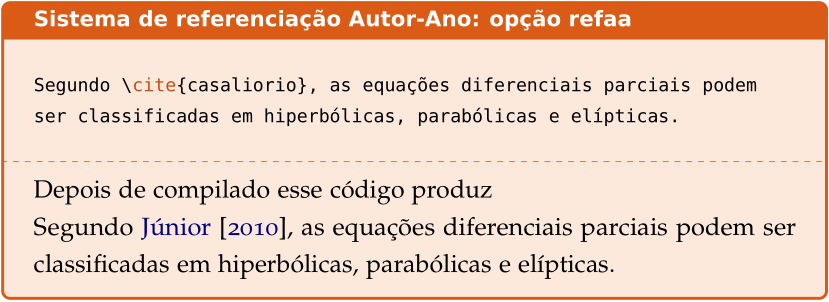
\includegraphics{Autor-Ano}}
\end{figure}

Observe que nos dois exemplos a citação é feita com o comando \cmc{cite}{casaliorio}, ou seja, é independente do estilo de bibliografia. Desta forma, para alterar a formatação de suas referências basta carregas um estilo diferente e compilar seu arquivo.

\subsubsection{Atenção}
Apenas as referências citadas no texto são incluídas na
lista de referências, ou seja, o \LaTeX\ previne esquecimentos
deliberados e impede que sejam incluídas nas referências
bibliografias que não foram citadas no texto.


\subsubsection{A lista de referências}

A lista de referências é criada na posição correspondente a inserção do comandos \com{bibliography} e sua primeira página recebe a mesma formatação da primeira página do sumário.

\section{Anexos e apêndices}
\begin{description}
\item[O que é um Anexo?]
	É um conjunto de informações complementares necessárias
    para a entendimento do trabalho ou parte dele.	
\item[O que é um Apêndice?]
	É um conjunto de informações suplementares acrescentado
    ao trabalho para suporte ou contextualização mas não
    necessário para o entendimento do trabalho ou parte dele.
\end{description}

\exemplo\,\, Seu trabalho usa fortemente resultados pouco conhecidos
ou extensos demais para serem inseridos no corpo do texto. No
final você pode inserir os tais resultados que constituirão um ou mais anexos.

\exemplo\,\, Seu trabalho aborda a vida de Charles Chaplin. No final você
pode inserir fotos de cartazes dos filmes dele, algumas de suas
frases famosas, fotografias dele. $\ldots$. Como essas informações
não são necessárias para o bom entendimento do seu trabalho elas
constituem um apêndice.

Note a diferença entre anexo e apêndice, o anexo contém informações
indispensáveis para a compreensão do trabalho enquanto o apêndice
contém informações acessórias e cuja ausência não comprometem a
compreensão do texto ou parte dele.

Na classe \estilo\ anexos são criados com o comando \com{anexo} e apêndices
são criados com o comando \com{apendice}, ambos utilizam o comando
\comando{appendix}, que é nativo da classe scrbook e não pode ser
carregado mais de uma vez no mesmo documento.

Para criar um anexo insira o comando \com{anexo}, depois dele todas
as ocorrêcias do comando \com{chapter} iniciarão um anexo.
\begin{tcolorbox}[title={Como criar anexos}]
	\begin{lstlisting}
	\anexo
	\chapter{Vida dura}
	\section{A vida gosta de quem gosta dela}
	\chapter{Você aprende}
	\section{Aprende que beijos não são contratos}
	\end{lstlisting}
	\tcblower
	
Depois de compilado esse código cria dois anexos: o Anexo I com
título Vida dura e a seção I.1 com título A vida gosta de quem gosta
dela, e o Anexo II com o título Você aprende e a seção II.1 com título
Aprende que beijos não são contratos
\end{tcolorbox}

Para criar um apêndice insira o comando \com{apendice},
depois dele todas as ocorrências do comando \com{chapter}
iniciarão um apêndice.
\begin{tcolorbox}[title={Como criar apêndice}]
	\begin{lstlisting}
	\apendice
	\chapter{Vida dura}
	\section{A vida gosta de quem gosta dela}
	\chapter{Você aprende}
	\section{Aprende que beijos não são contratos}
	\end{lstlisting}
	\tcblower
	
Depois de compilado esse código cria dois apêndices: o
Apêndice A com título Vida dura e a seção A.1 com título A
vida gosta de quem gosta dela, e o Apêndice B com o título
Você aprende e a seção B.1 com título Aprende que beijos
não são contratos
\end{tcolorbox}
\subsection{Apêndice sem anexo}
O apêndice deve vir depois do anexo. Para atender a essa norma
o comando \com{apendice} foi implementado de modo que só
funciona corretamente depois do comando \com{anexo}. Se
acontecer de o trabalho exigir apenas a inclusão de apêndices
deve-se carregar a opção de classe \ttt{apenas} e utilizar o
comando \com{apendice} normalmente para criar os apêndices.


%%%
%%%\backmatter %%% Apesar de pertencer à classe scrbook, não o use na estilo.
%%%
\nocite{*}  %%% insere todos os itens do arquivo .bib na lista de referências,
            %%% independente de eles serem citados no texto.
\addcontentsline{toc}{chapter}{Referências}  %%% Só para a opção glenn
\renewcommand{\bibname}{Referências}         %%% Para contornar o babel.
\bibliographystyle{unsrtnat}
\bibliography{bibliografia}   %%% Insere o arquivo bibliografia.bib que deve
                              %%% ficar na mesma paste de seu arquivo tex.

\anexo
\chapter{Deus}

\section{Seja grato}
Tu sempre foste meu melhor amigo, Aquele que nunca me abandonou 
ou desamparou; e por tudo isso Te agradeço, meu Deus!


Só Deus é digno de toda a honra, glória e louvor!

Em primeiro lugar, devemos louvar a Deus porque Ele merece. O nosso louvor não pode depender das nossas emoções, porque as nossas emoções mudam, mas Deus é sempre igual.


\chapter{A vida}

A vida gosta de quem gosta dela e quem tem quem lhe chore morre todo dia.

\section{Você aprende}

Aprende que falar pode aliviar dores emocionais, e descobre que se leva anos para se construir confiança e apenas segundos para destruí-la, e que você pode fazer coisas em um instante, das quais se arrependerá pelo resto da vida; aprende que verdadeiras amizades continuam a crescer mesmo a longas distâncias, e o que importa não é o que você tem na vida, mas quem você tem na vida, e que bons amigos são a família que nos permitiram escolher.

Aprende que não temos que mudar de amigos se compreendemos que eles mudam; percebe que seu melhor amigo e você podem fazer qualquer coisa, ou nada, e terem bons momentos juntos.

Descobre que as pessoas com quem você mais se importa na vida são tomadas de você muito depressa, por isso sempre devemos deixar as pessoas que amamos com palavras amorosas; pode ser a última vez que as vejamos.

E descobre que não importa o quanto você se importa, algumas pessoas simplesmente não se importam.

Aprende que não importa em quantos pedaços seu coração foi partido, o mundo não pára para que você o conserte.

Portanto$\ldots$ plante seu jardim e decore sua alma, ao invés de esperar que alguém lhe traga flores.


\apendice
\chapter{Um teste de apêndice}

\section{Diferenças}

\subsection{Anexo}
Seu trabalho usa fortemente resultados pouco conhecidos
ou extensos demais para serem inseridos no corpo do texto. No
final você pode inserir os tais resultados, a coleção deles
constitui-se um ou mais anexos.

\subsection{Apêndice}

Seu trabalho aborda a vida de Charles Chaplin. No final você
pode inserir fotos de cartazes dos filmes dele, algumas de suas 
frases famosas, fotografias dele, citar um poema ou parte dele $\ldots$. 
Como essas informações não são necessárias para o bom entendimento do 
seu trabalho elas constituem um apêndice.


Note a diferença entre anexo e apêndice, o anexo contém informações 
indispensáveis para a compreensão do trabalho enquanto o apêndice 
contém informações acessórias e cuja ausência não comprometem a 
compreensão do texto ou parte dele.

\section{Erro}
pdftex warning (ext4): destination with the same identifier has been already used, duplicate ignored


\chapter{A vida continua}
\section{Você}

Depois de um tempo você aprende que o sol pode queimar se ficarmos expostos a ele durante muito tempo. E aprende que não importa o quanto você se importe: algumas pessoas simplesmente não se importam$\ldots$. E aceita que não importa o quão boa seja uma pessoa, ela vai ferí-lo de vez em quando e, por isto, você precisa estar sempre disposto a perdoá-la.


\end{document}
